\section{Simulation examples}

In the end, the purpose of this project is to produce animations for computer graphics, and the
last word must be given to the human observer who watches these animations. I would like to claim
that the results are of a quality similar to what an animator might create, and that they are
realistic in the sense that they do not violate the laws of physics or anatomy. However, such a
claim is difficult to defend convincingly in print. I have therefore compiled a video of several
example animations, and I urge the reader to watch it to gain a more personal impression of this
project's results. The video can be found in the 3D graphics section of my web site
\texttt{http://martin.kleppmann.de/}. The following sections describe how each of the simulated
systems was implemented and point out noteworthy features.

\subsection{Pendulum systems}

The simplest physical system in the demonstration video is
the animation of a double pendulum (a rigid pendulum with a second one
attached to its end), and its extension to three, eight and 25 segments. The double pendulum is
a commonly studied system in physics; although it does not have an exact analytic solution, an
approximate solution can be found for small angles. In this case, one finds that the resulting
movement is the sum of two simple harmonic oscillations at different frequencies, resulting in
a mysterious-looking swinging movement.

The double, triple and eight-part pendulums are set up in a very similar way. Each segment is
modelled as a rigid cylinder with constant density. The top end of the top segment is held in
place by a `nail' constraint. Each pair of adjacent segments is connected by a ball-and-socket
joint. Initially, all segments are at rest, the first segment is rotated by 45 degrees
anticlockwise from the equilibrium position, and all other segments hang straight down.

The simulation does not employ an XML input file; instead, the objects representing the bodies
and the constraints are directly created by the Java test case. The simulation results were
exported to Blender and rendered using the internal renderer and orthographic projection.
I also performed a Fourier transform on the results of the double pendulum simulation, which
indicated very clearly that there were two main frequency components.

The 25-segment pendulum is an attempt to simulate rope, and it is considerably more ambitious.
It is modelled as a cylindrical mesh bound to a chain of 25 bones. The ground is a separate mesh,
and in the simulation its position is fixed by three `nail' constraints. This input data is
represented as an XML file. Collision detection is performed on basis of the meshes, thus the
rope can collide both with itself and with the ground.

The joints between adjacent segments of the rope are of ball-and-socket type, and their rotation
is limited to a maximum of 15 degrees about each axis. The si\-mu\-la\-ted rope is therefore very
stiff. I am not entirely sure how realistic I should consider this simulation; its behaviour looks
strange at first, but this is mainly due to the assumptions put into the model. I believe that
the simulation correctly obeys the model, but the model would have to be refined in order
to produce genuinely realistic-looking rope.

\subsection{Newton's cradle}

\begin{figure}[p]
\centerline{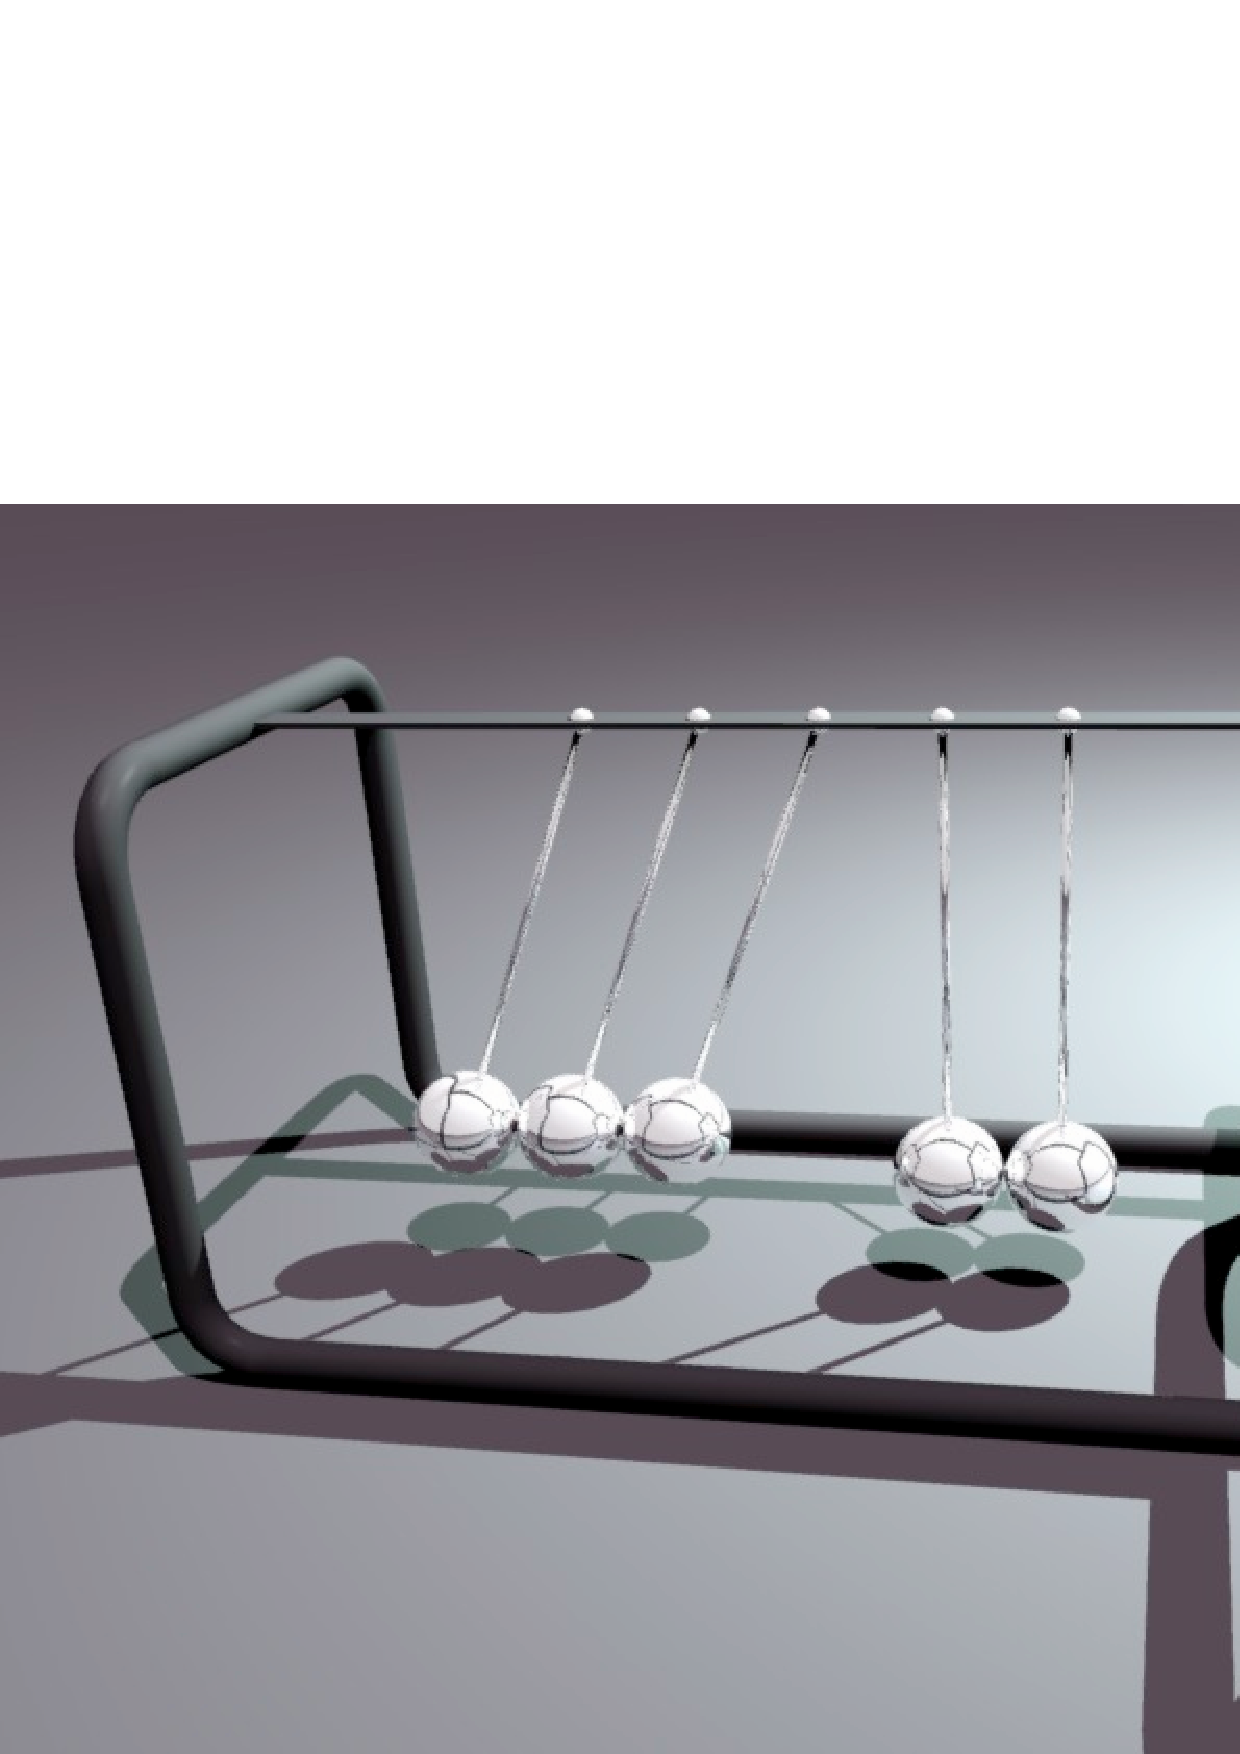
\includegraphics[width=60mm,height=45mm]{figures/cradle1} \hspace{5mm}
            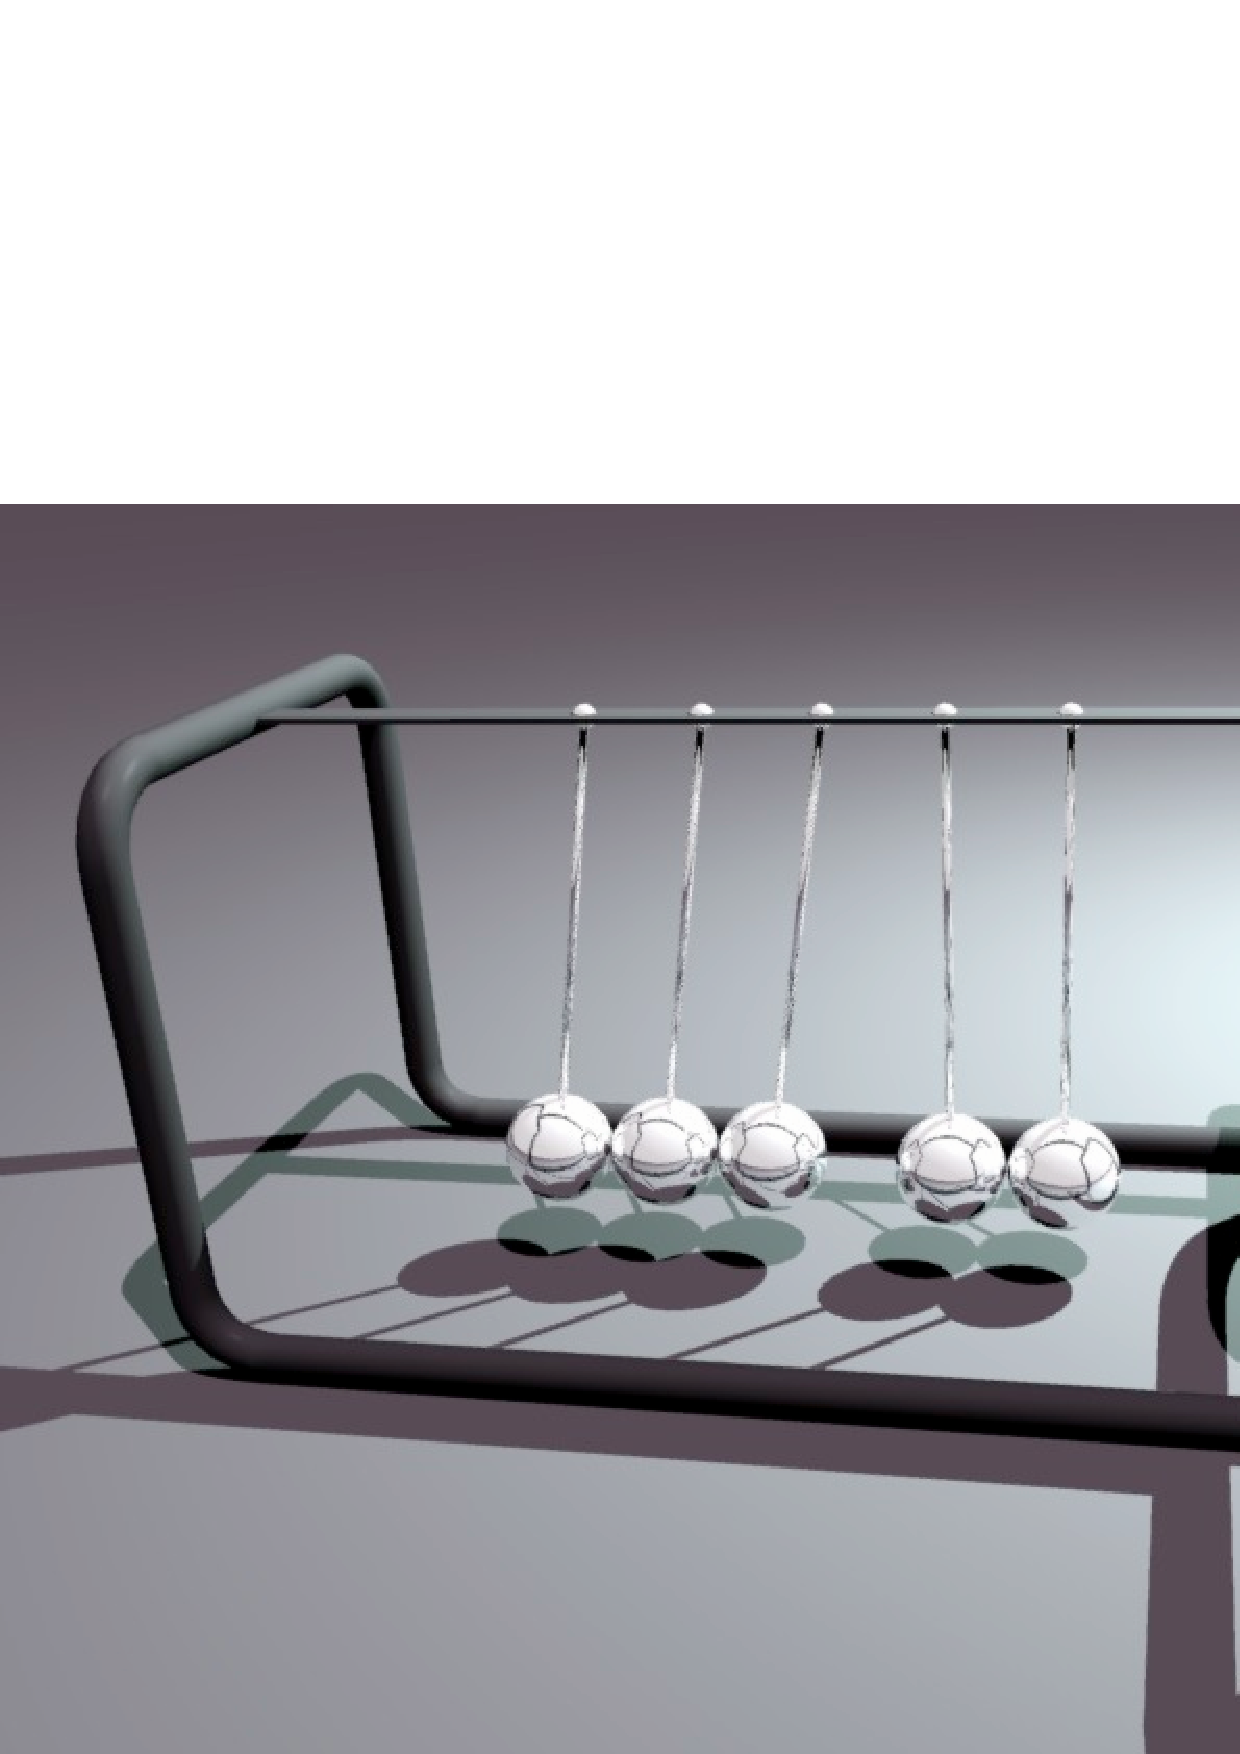
\includegraphics[width=60mm,height=45mm]{figures/cradle2}}\vspace{5mm}
\centerline{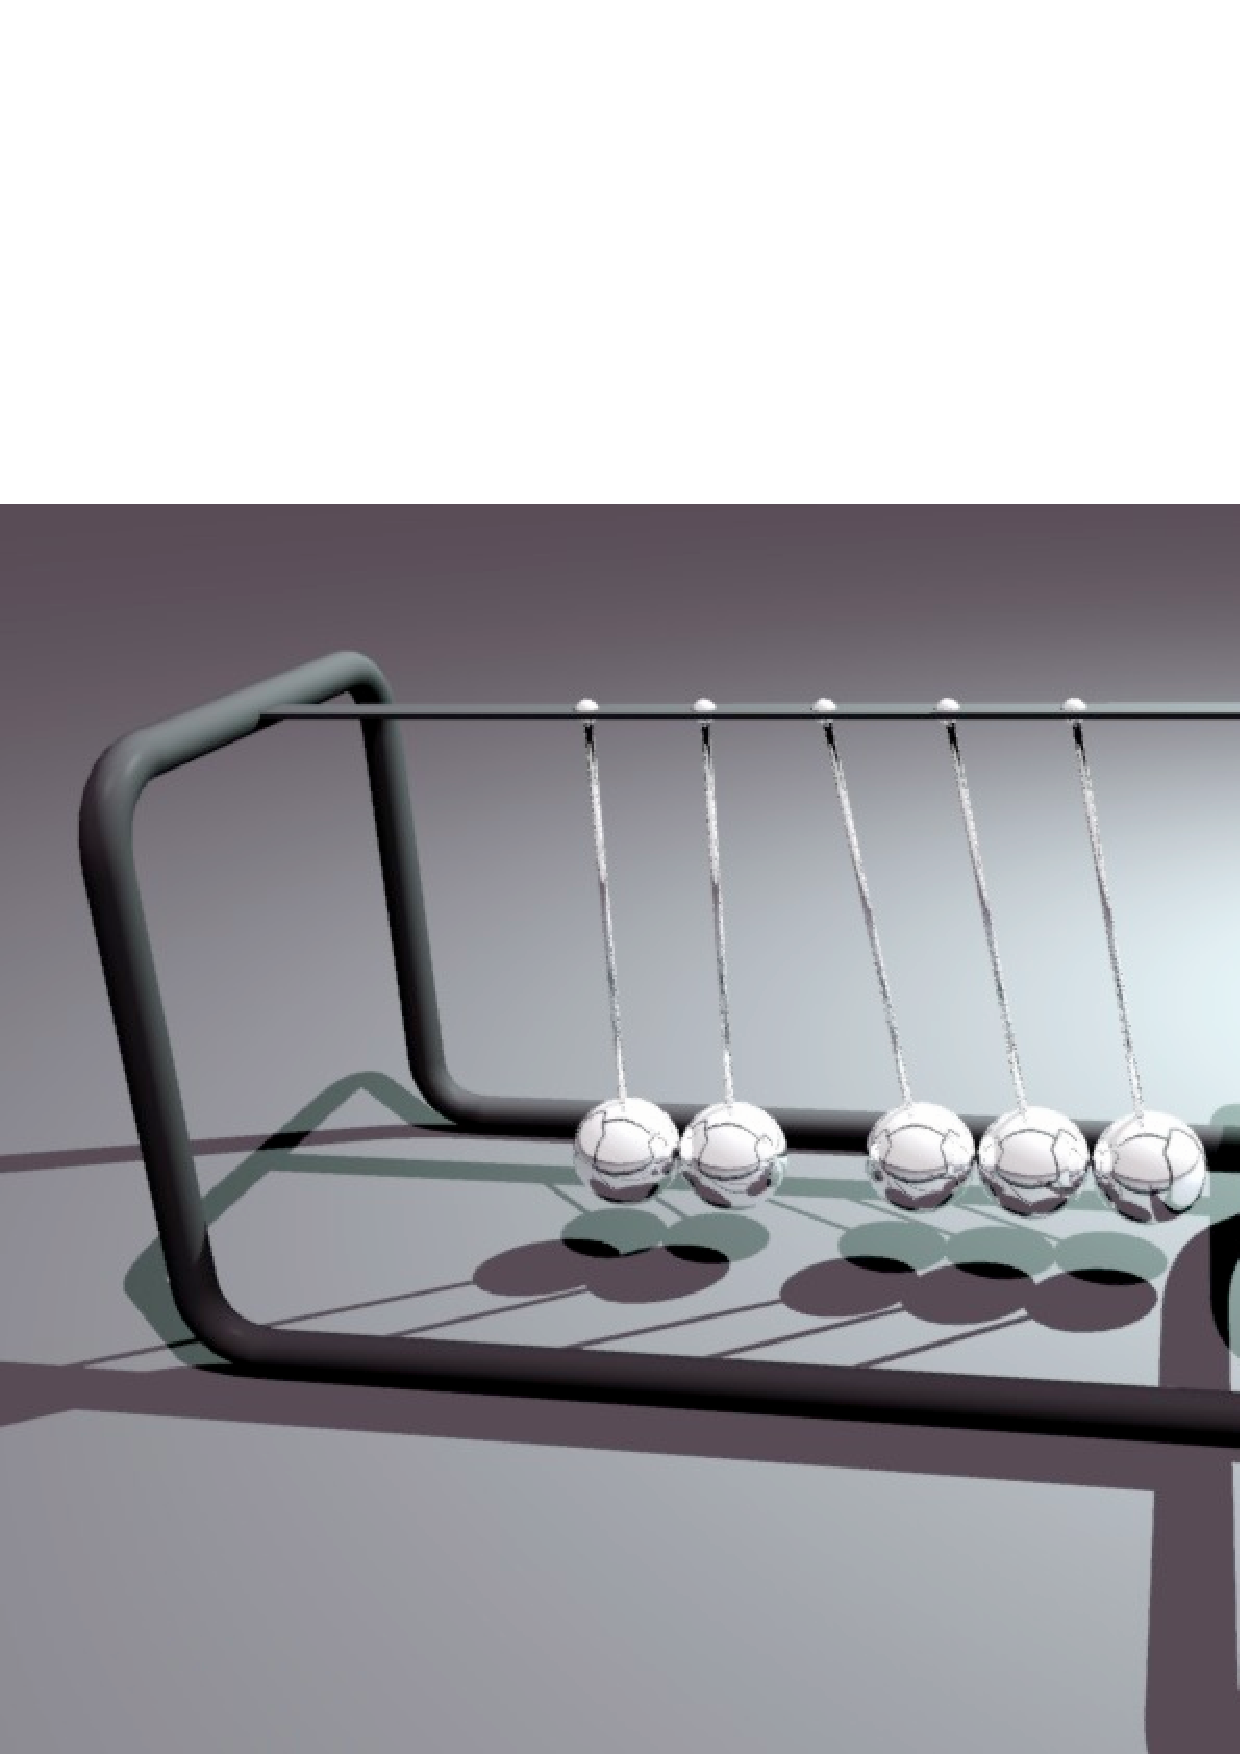
\includegraphics[width=60mm,height=45mm]{figures/cradle3} \hspace{5mm}
            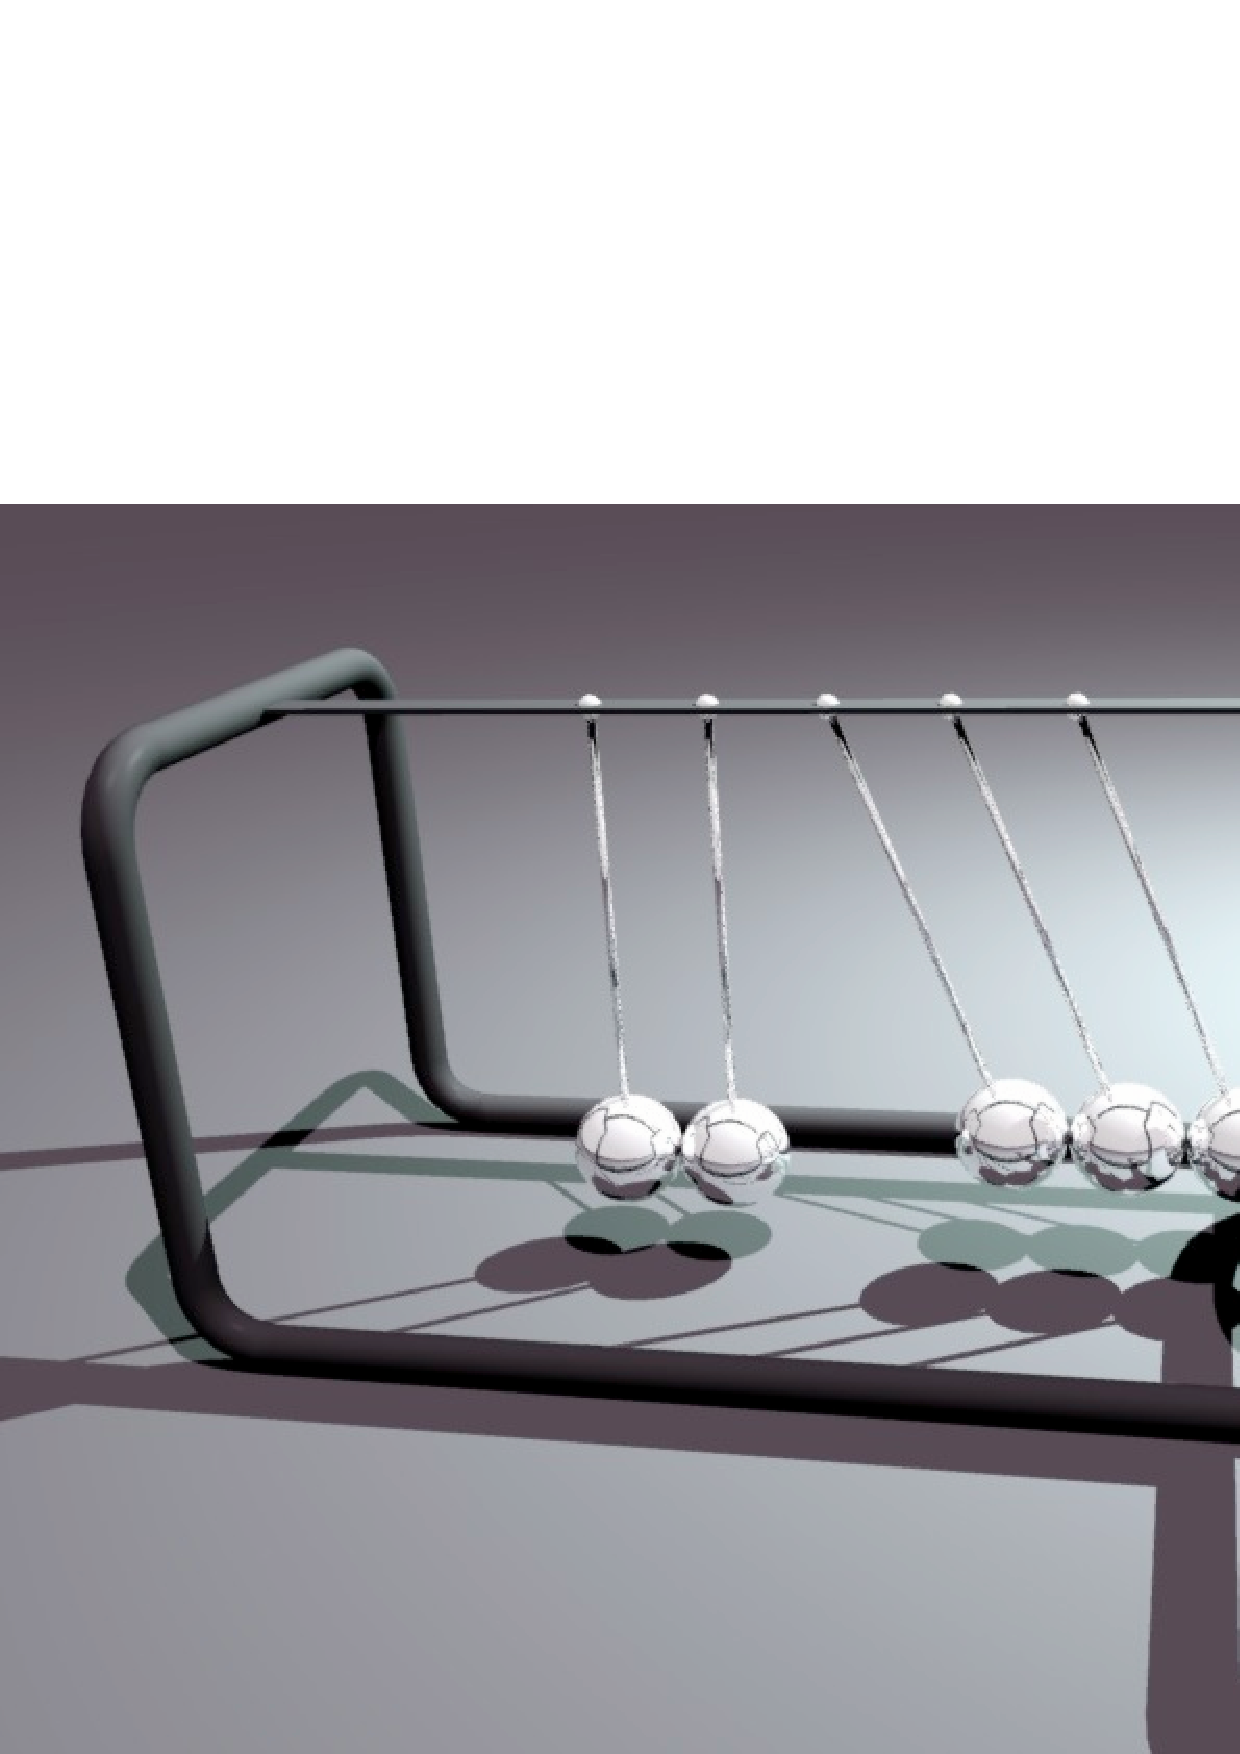
\includegraphics[width=60mm,height=45mm]{figures/cradle4}}
\caption{Animation of Newton's cradle.\label{sampleCradle}}
\end{figure}

The next section shows Newton's cradle in a range of different animations. For full elasticity,
various combinations of one, two and three balls in simultaneous motion are demonstrated, and all
effects observed in a real toy cradle are reproduced. I also simulate what happens if collisions
are not fully elastic: all balls gradually begin to swing, and the sequence of collisions becomes
much more complicated.

Newton's cradle is modelled as five spherical bodies, each with its centre of mass at the centre
of the ball (i.e.\ the wire connecting it to the frame is assumed to be massless). The joint to
the frame is modelled as a `nail' constraint, and the frame itself does not exist in the
simulation. Collision detection is performed not on the basis of the meshes (since these are
polyhedral approximations and not exact spheres), but using a special type of sphere/sphere
constraint which computes its behaviour using the positions of the centres of the balls and their
radii.

For the simulation to work accurately, a very low penetration tolerance must be set. The different
examples are simulated in exactly the same way, independent of the number of balls moving or the
elasticity of collisions.

\subsection{Falling boxes}

\begin{figure}[p]
\centerline{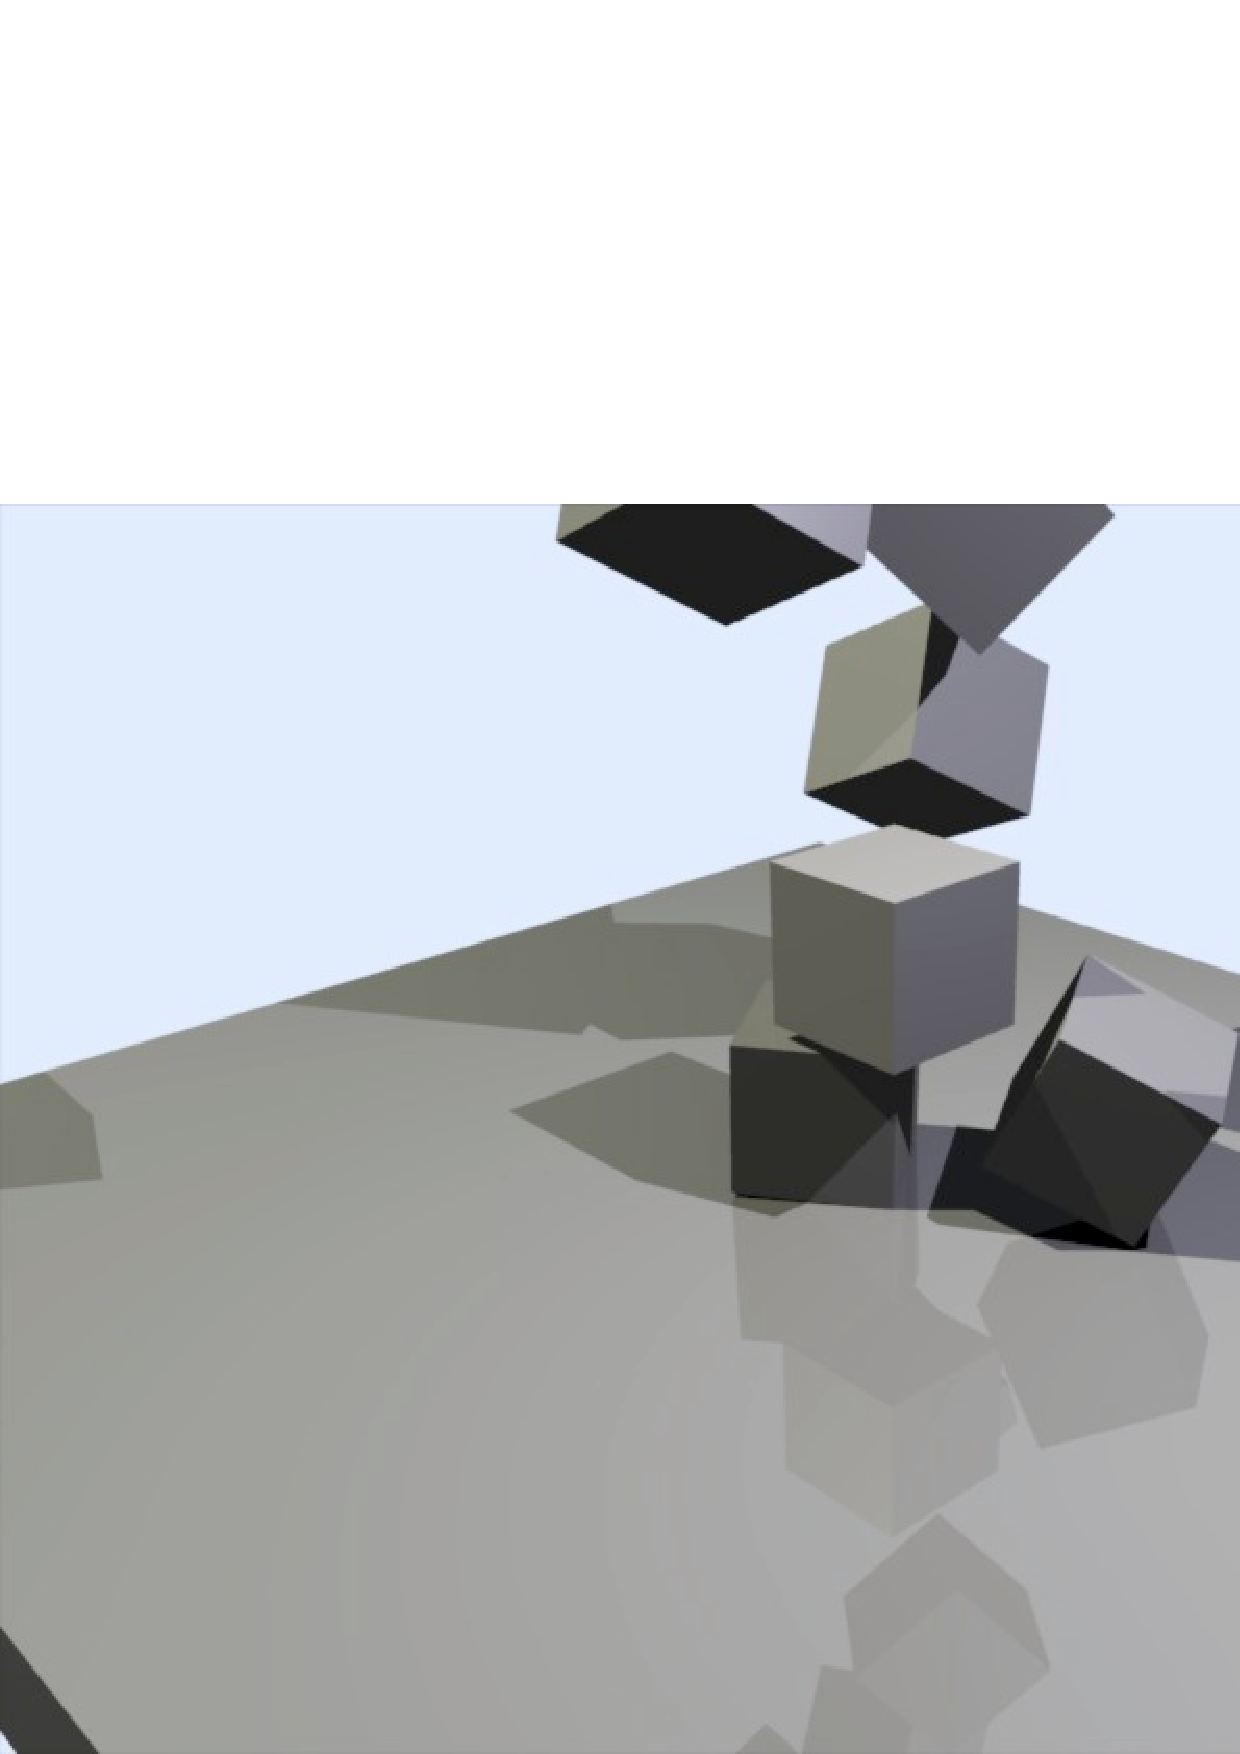
\includegraphics[width=60mm,height=45mm]{figures/boxes1} \hspace{5mm}
            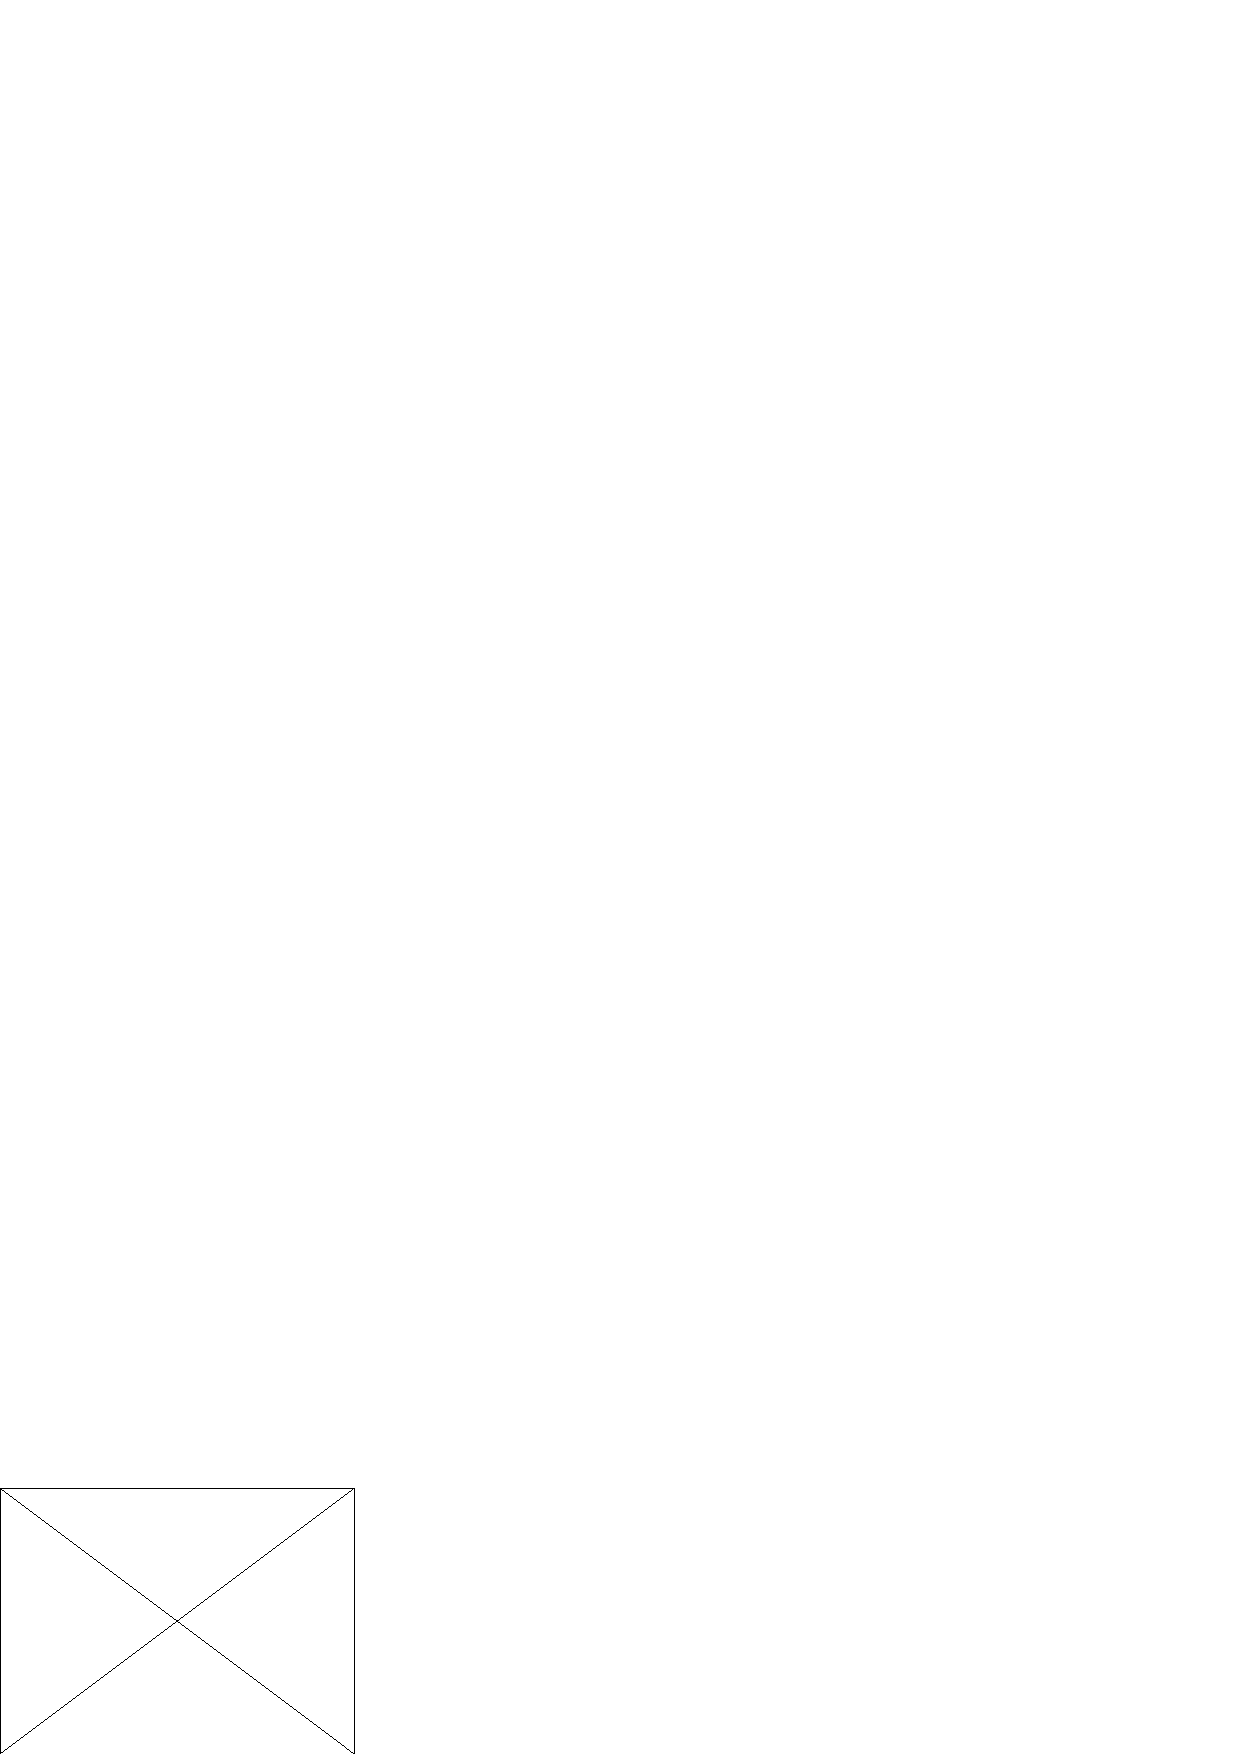
\includegraphics[width=60mm,height=45mm]{figures/boxes2}}\vspace{5mm}
\centerline{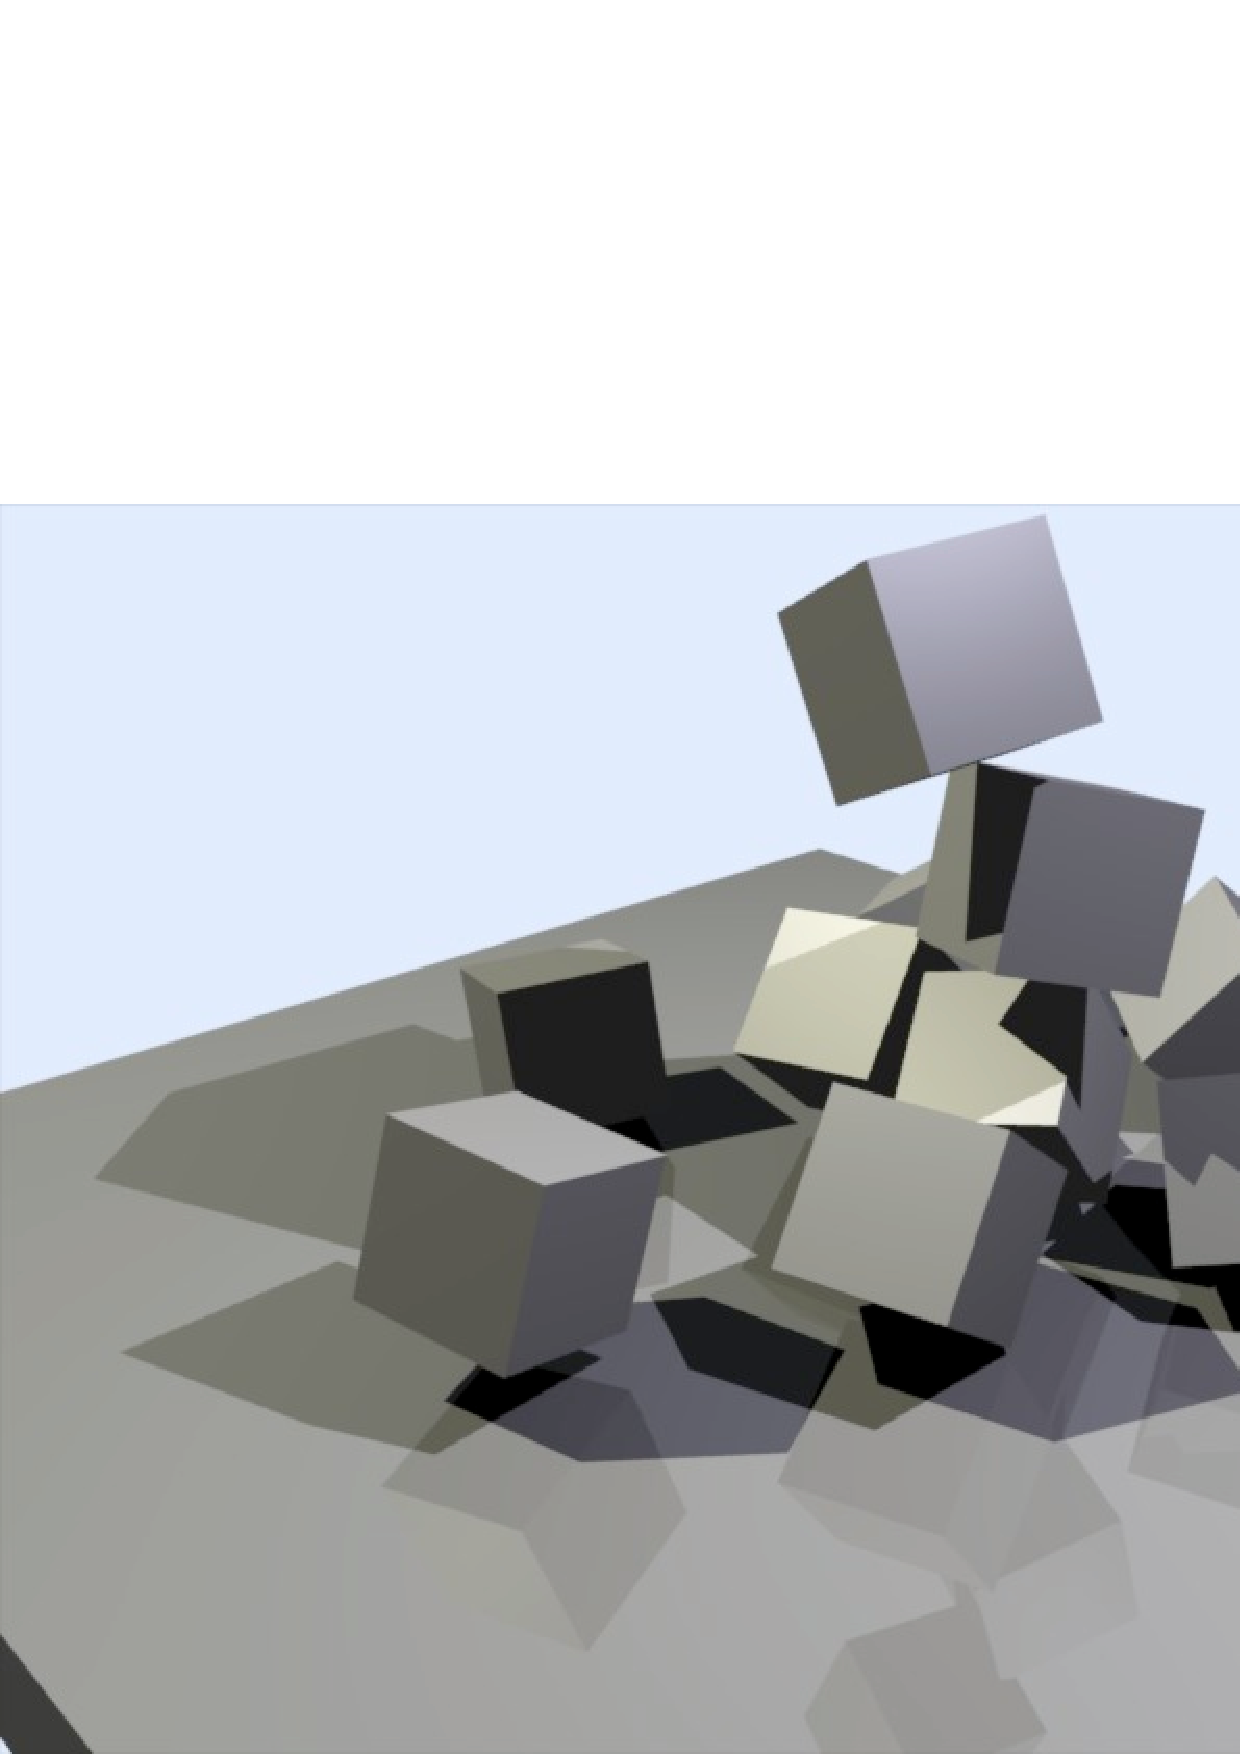
\includegraphics[width=60mm,height=45mm]{figures/boxes3} \hspace{5mm}
            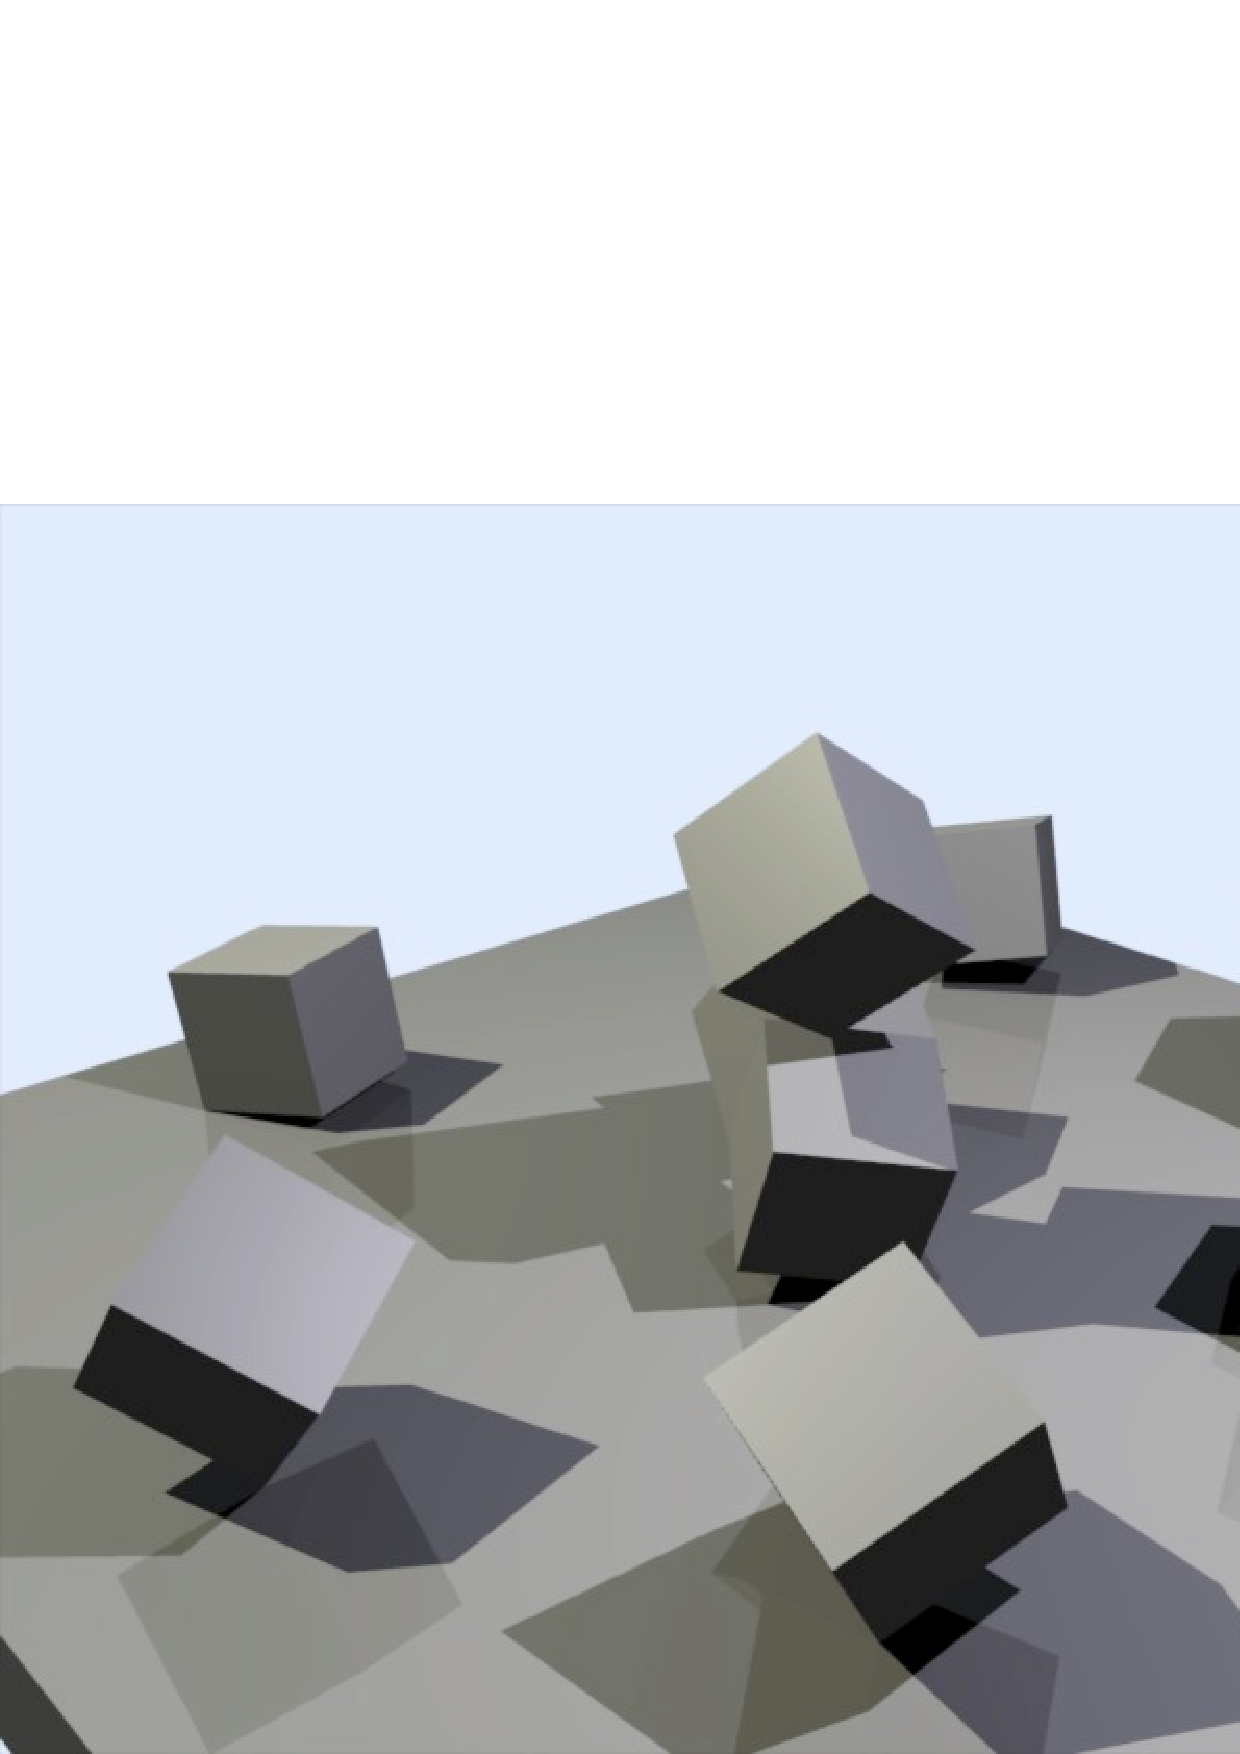
\includegraphics[width=60mm,height=45mm]{figures/boxes4}}
\caption{Animation of ten boxes falling onto a table.\label{sampleBoxes}}
\end{figure}

The third section demonstrates eleven interacting rigid bodies: ten boxes falling onto a table.
The simulation is performed at two different elasticities: one close to what one would expect in
reality ($\varepsilon = 0.2$), and one very bouncy as contrast ($\varepsilon = 1.0$).

Each of the ten boxes is modelled as a symmetric hollow body. All boxes and the table are
specified as meshes in an XML input file. The table is held in place by three `nail' constraints.
These simulations exhibit a range of different collision types: each example starts with a
vertex/face collision when the first box hits the table, and is followed by a sequence of
vertex/face, edge/edge and compound collisions. Whenever a collision cannot be clearly classified
as either vertex/face or edge/edge, the algorithm searches for a plane which contains as closely
as possible the line of intersection between the two colliding meshes. This plane is then used as
the contact plane for computing the impulses and resting contact forces.

The fully elastic version of this simulation looks unrealistic because it behaves as though the
boxes were made of extremely bouncy rubber. The version with elasticity 0.2 is much closer to what
one might expect in a real-life scene, but the contrast between the two is interesting. At the
end of the low-elasticity simulation, several boxes can be seen in a frictionless glide over the
surface of the table. They cannot penetrate the table due to a resting contact force.

\subsection{Alfred falling down stairs}

The final two sections show a humanoid model fall down a straight staircase and a spiral staircase
respectively. I created these simulations to demonstrate a situation which did not require control
of muscular forces (which are hard to control in a simulation~\cite{Green:91}) but were
nevertheless interesting.

The simulation on straight stairs and on the spiral staircase are set up in a very similar way.
Each scene consists of two bodies, a polygon model of the staircase and Alfred himself. In each
case, the staircase is held in place by three `nail' constraints\footnote{It seems intuitively
bizarre that one might make a whole staircase immobile by only three nails, but in the simulation
the magnitude of the forces is, of course, almost irrelevant!}. Alfred is an articulated body
as described in section~\ref{softwareTools}.

All meshes and skeletons are defined in an XML input file. All joints' rotation is restricted in
a way which approximates the anatomical reality. Nonetheless the body sometimes enters poses which,
although they are not impossible, look rather uncomfortable. This is because a pose does not
gradually become more uncomfortable as the limit is approached, but action takes place only at
the limit. The articulated body model would have to be extended to accommodate a notion of
``comfort'' or elastic limits.

For purposes of collision detection, the shape of the Alfred mesh is approximated by 252 little
spheres. The staircase is not approximated. Thus this simulation does not make use of the usual
vertex/face and edge/edge collisions; instead, sphere/face and sphere/edge collisions occur
(on contact with the staircase), and sphere/sphere collisions (on contact between different parts
of the articulated body, e.g.\ the hand against the chest). I found the use of spheres to be the
most reliable technique for such a complicated mesh. Constraint functions for these types of
collision can be derived fairly easily and handled using the usual algorithms for resting and
colliding contact as described in section~\ref{collisionHandling}.

The camera movement and lighting was set up in Blender. After importing the simulation results,
the animation was rendered using Blender's internal renderer/raytracer. Some of the mesh
deformations look strange; this is unrelated to the simulation, but must be blamed on my lack of
3D art skills!

\begin{figure}[p]
\centerline{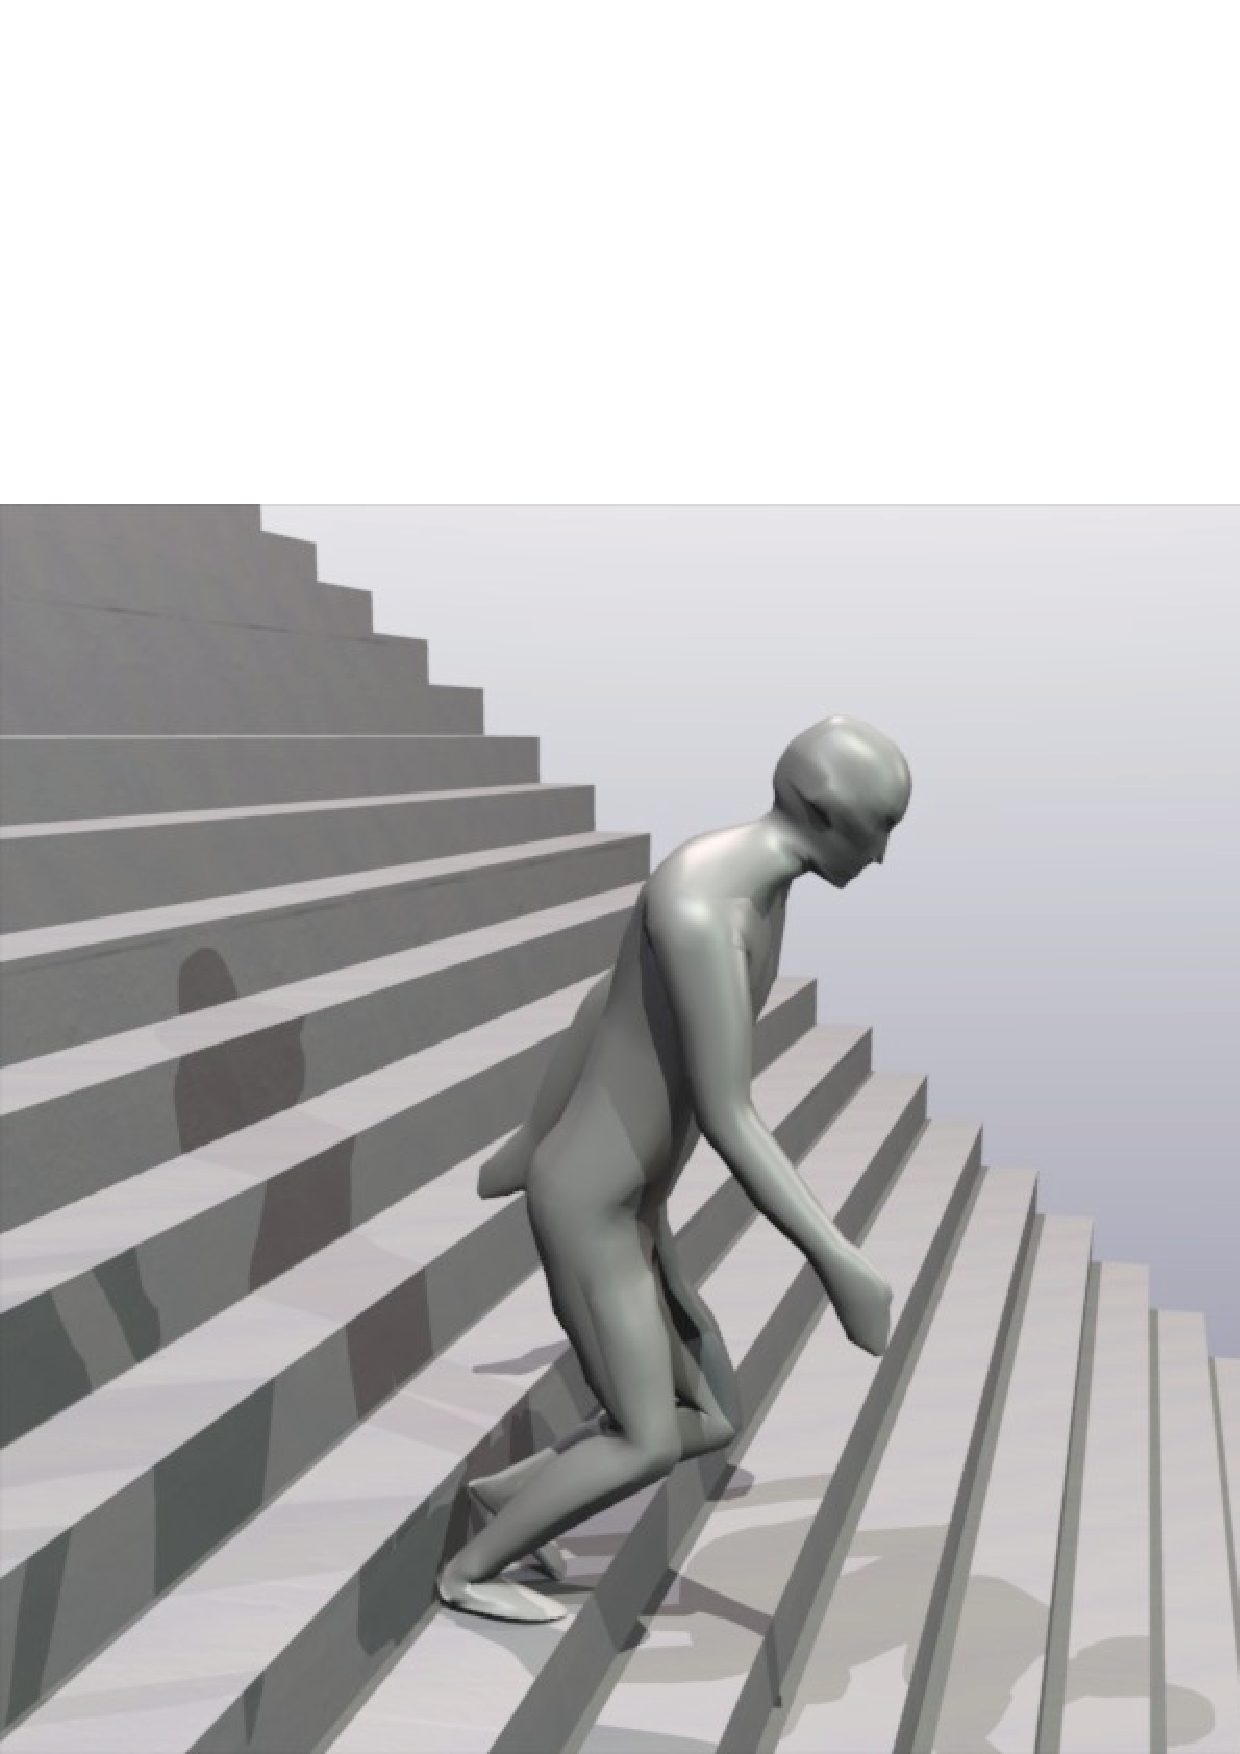
\includegraphics[width=60mm,height=45mm]{figures/stairs1} \hspace{5mm}
            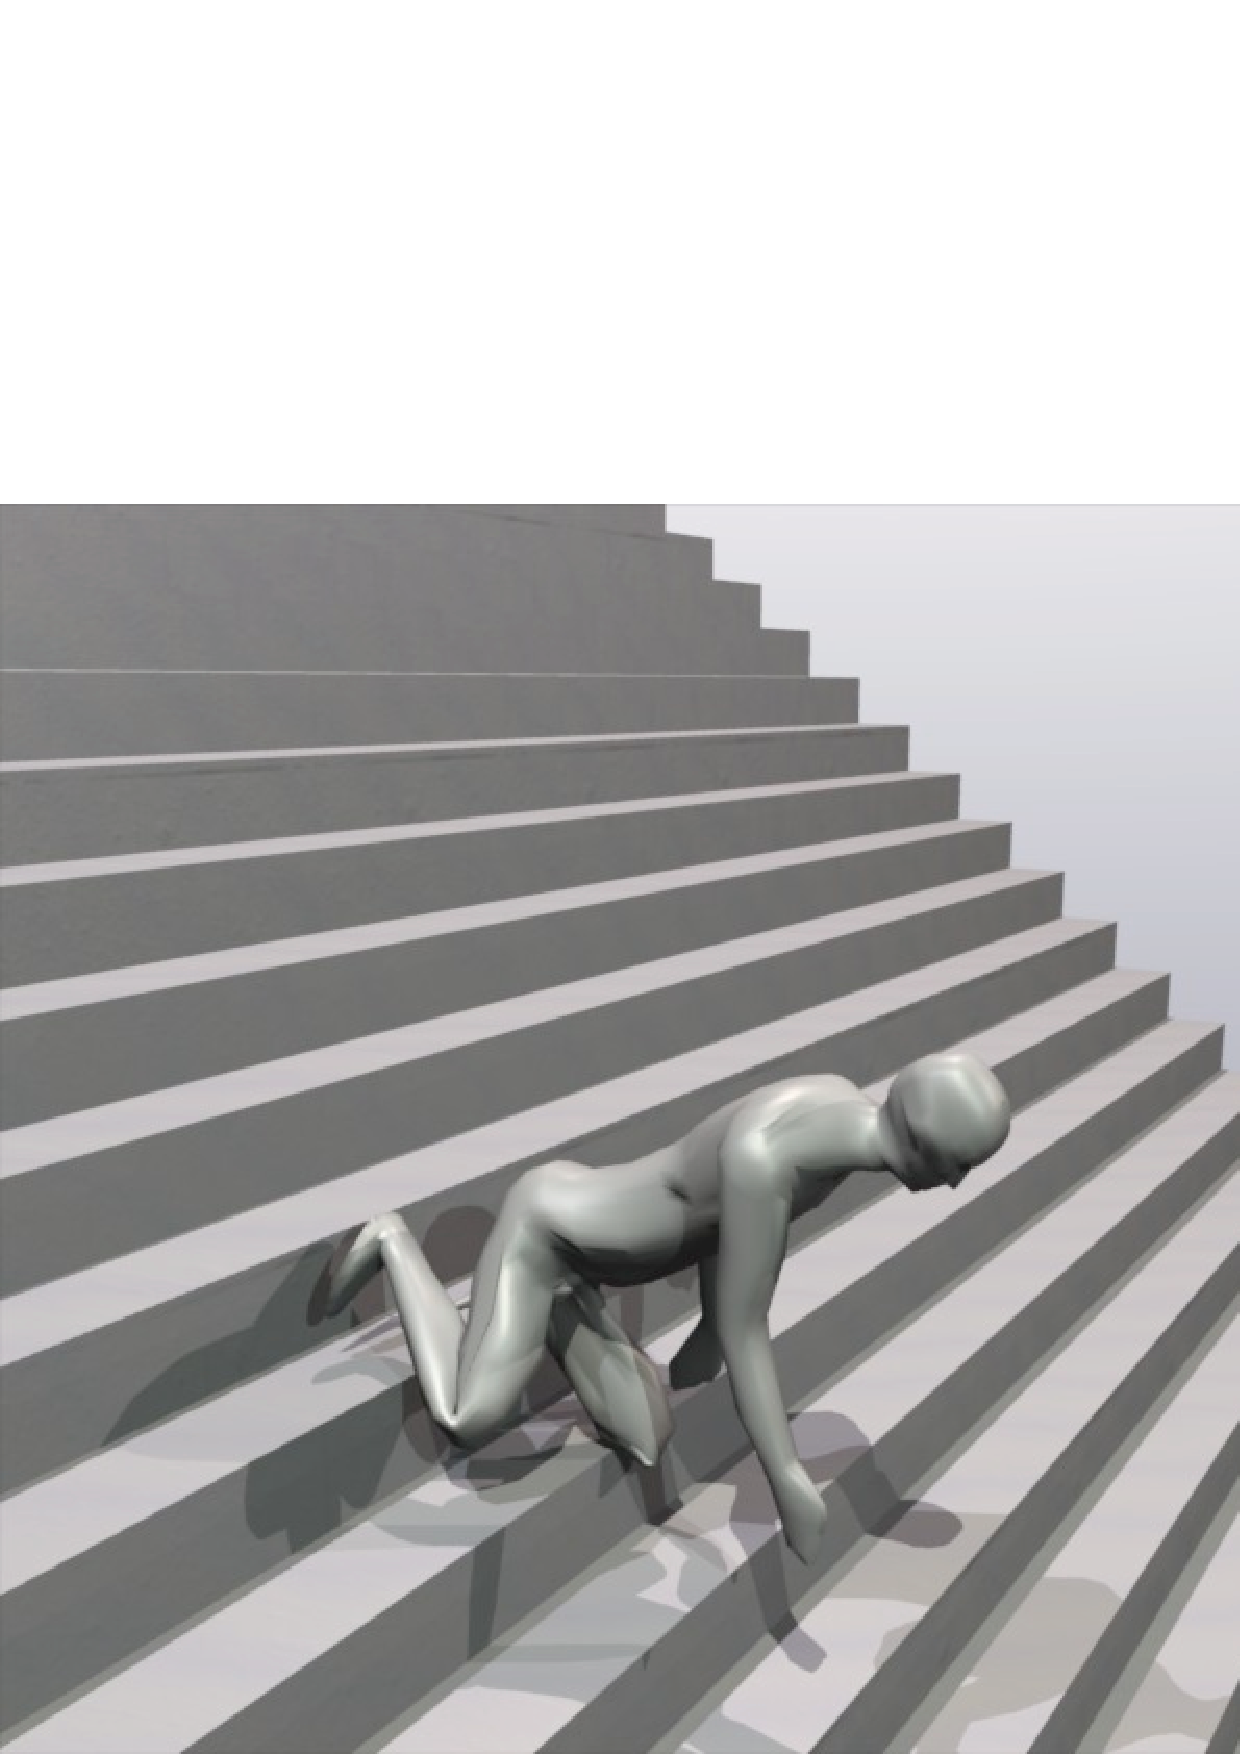
\includegraphics[width=60mm,height=45mm]{figures/stairs2}}\vspace{5mm}
\centerline{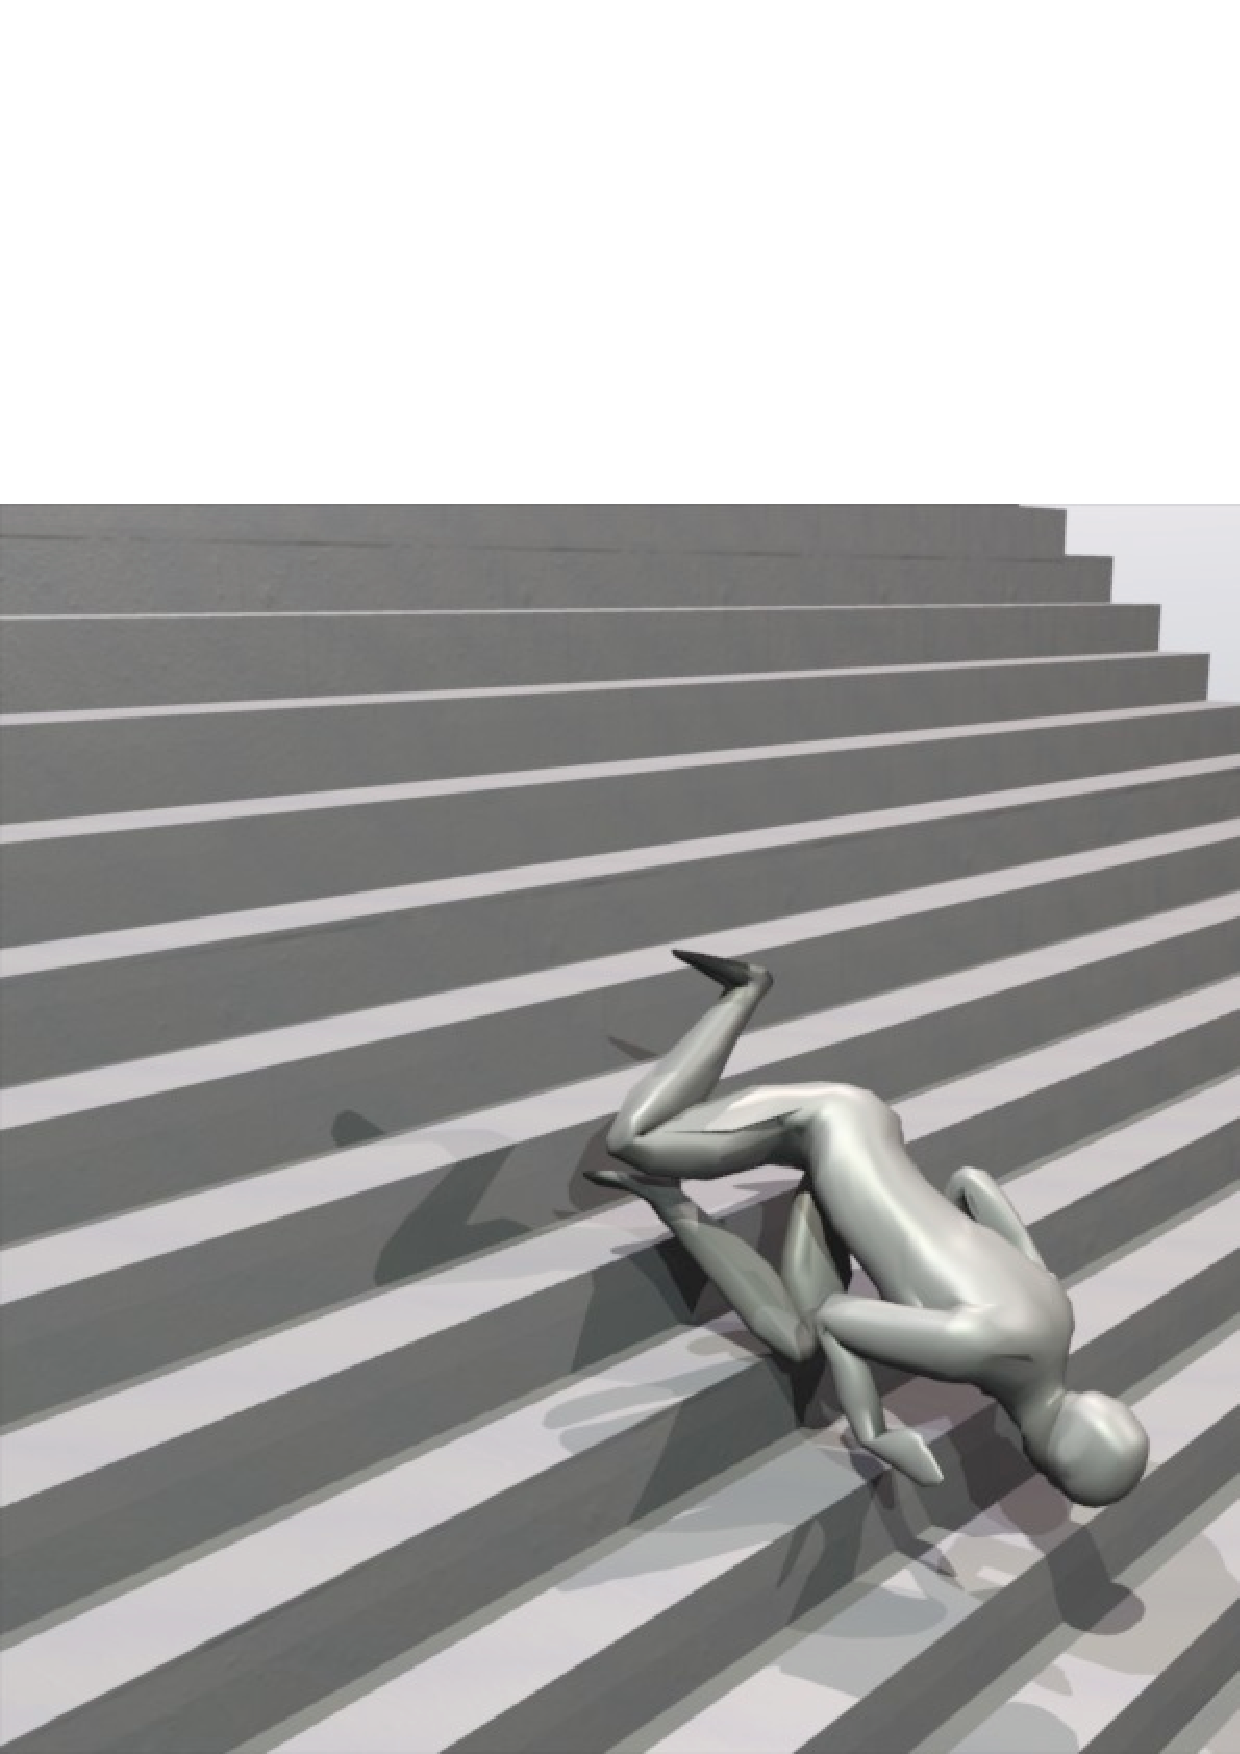
\includegraphics[width=60mm,height=45mm]{figures/stairs3} \hspace{5mm}
            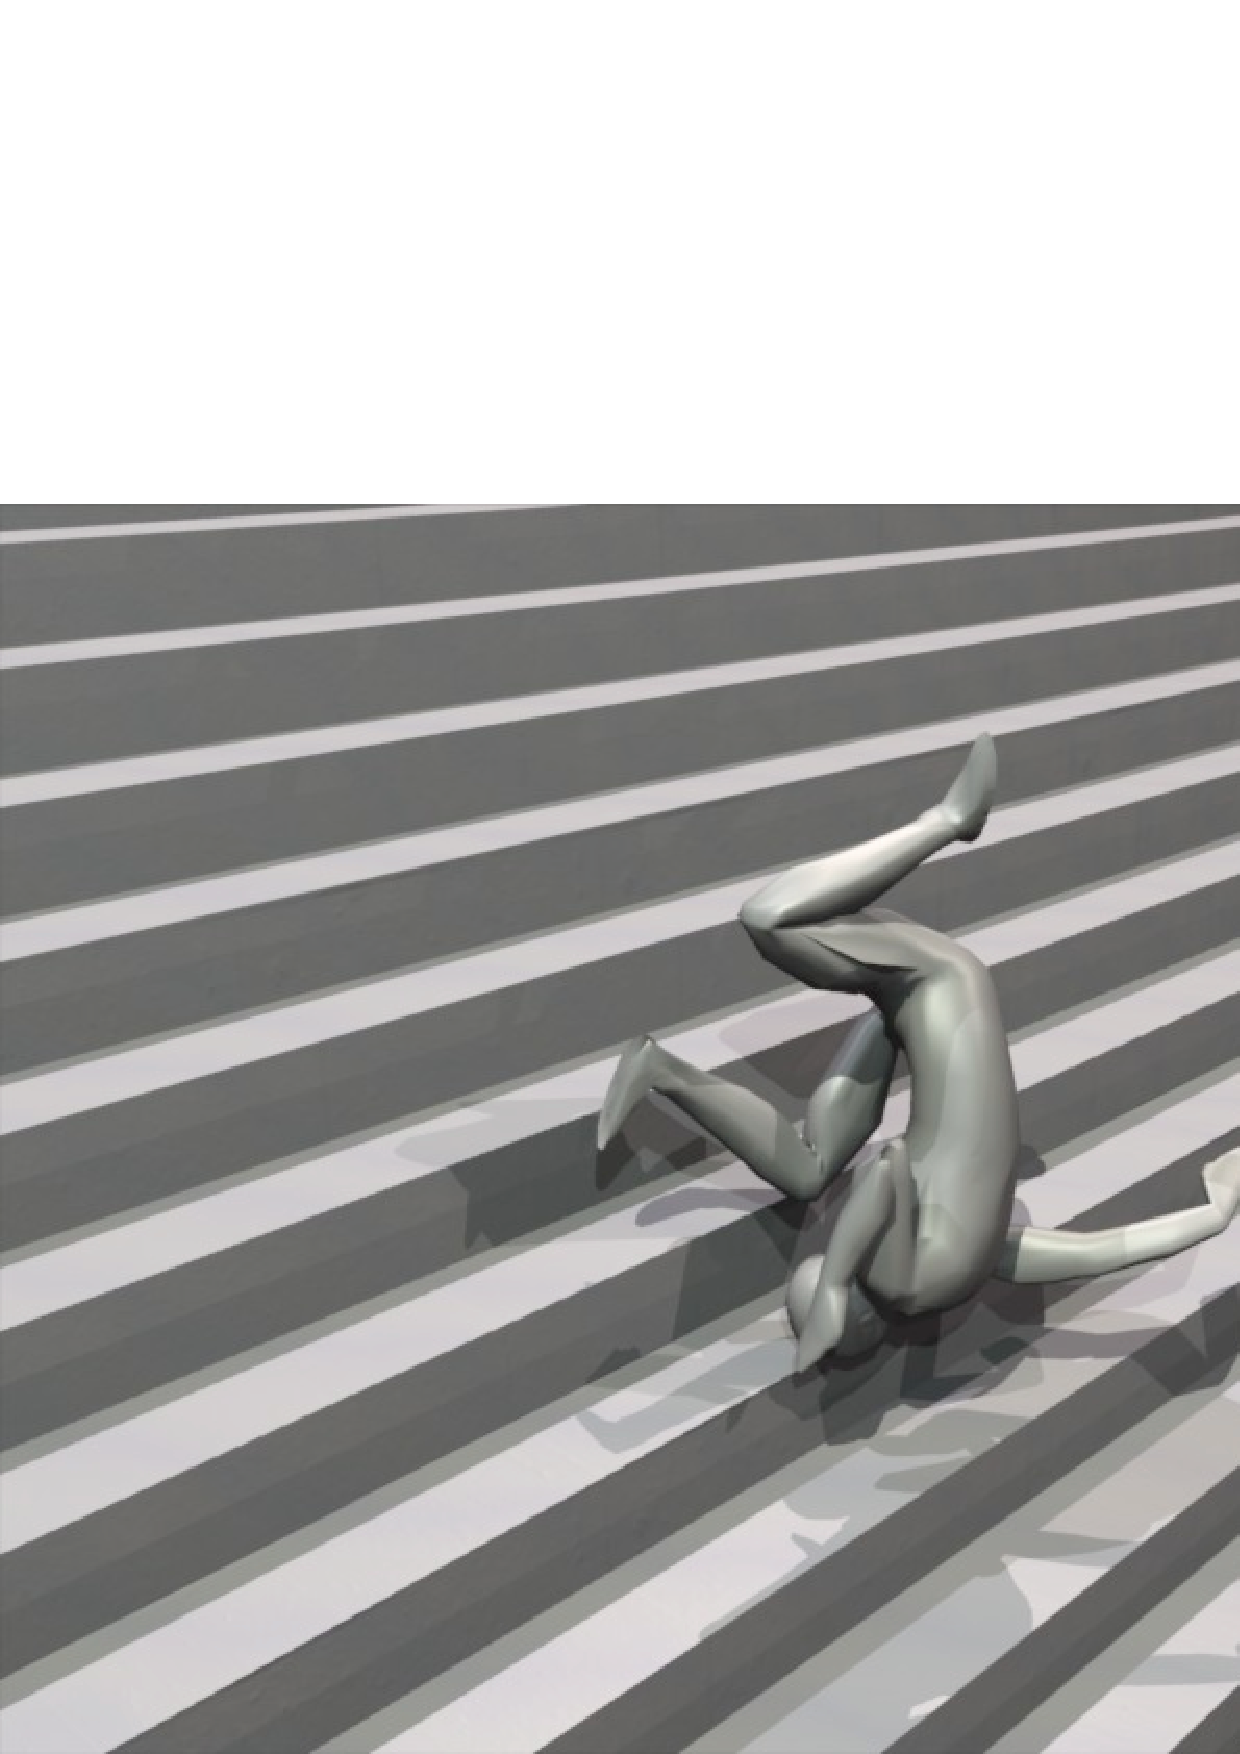
\includegraphics[width=60mm,height=45mm]{figures/stairs4}}
\caption{Animation of Alfred falling down a set of stairs.\label{sampleStairs}}
\end{figure}

\begin{figure}[p]
\centerline{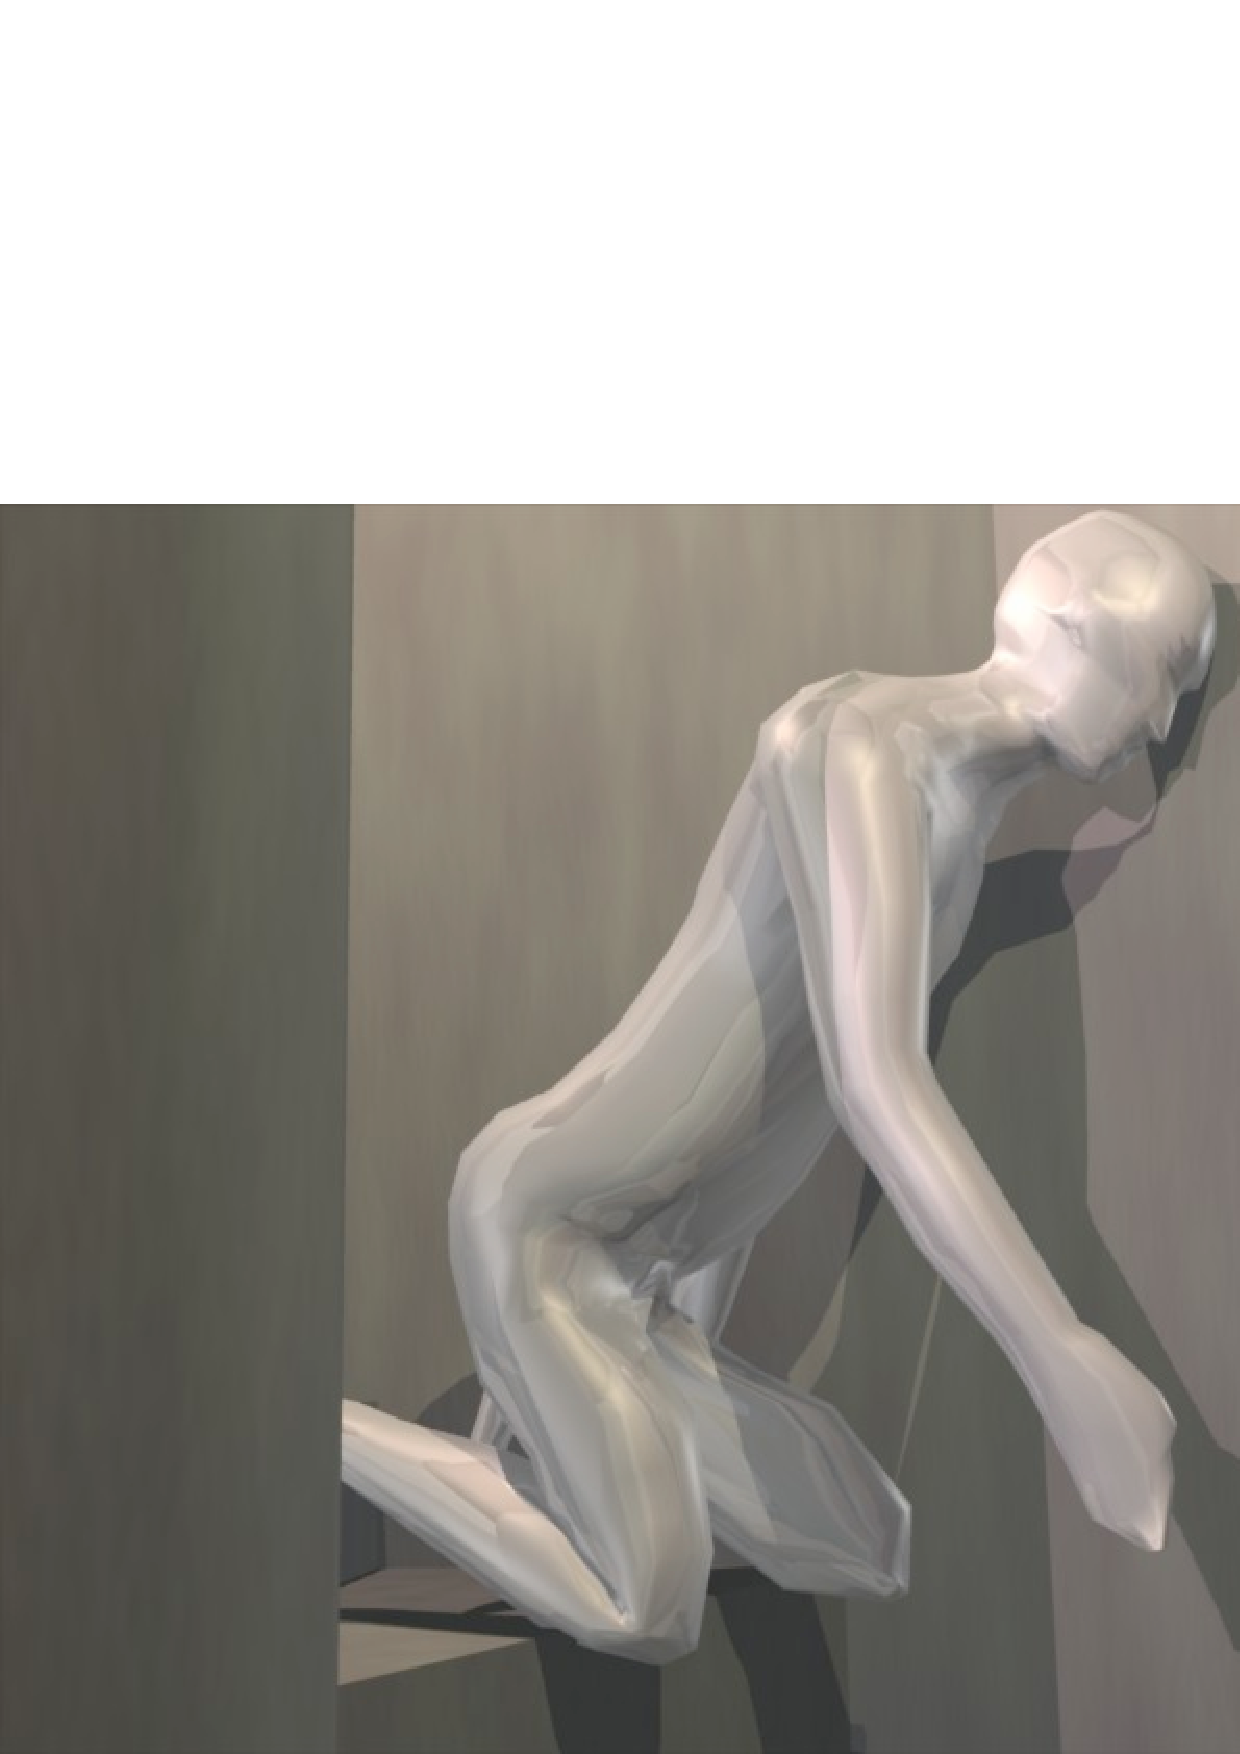
\includegraphics[width=60mm,height=45mm]{figures/spiral1} \hspace{5mm}
            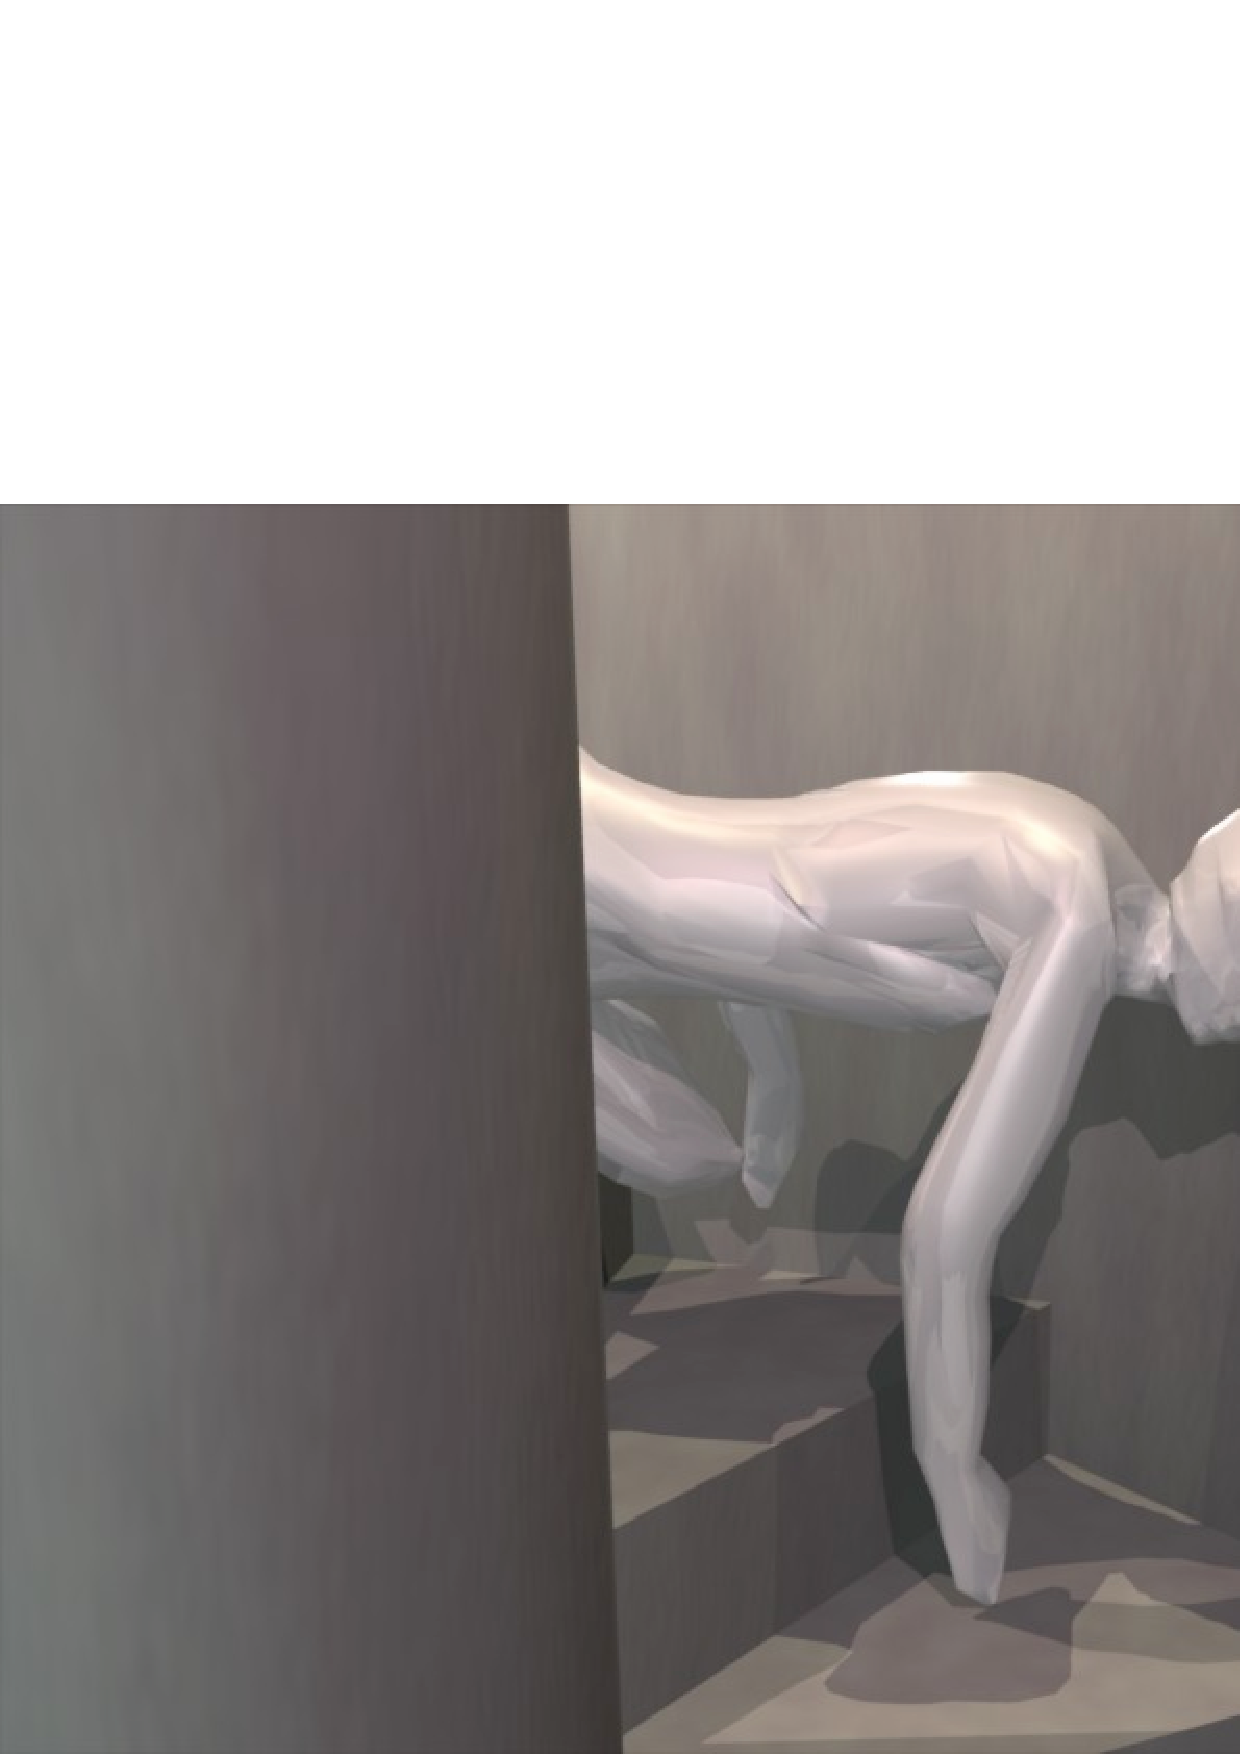
\includegraphics[width=60mm,height=45mm]{figures/spiral2}}\vspace{5mm}
\centerline{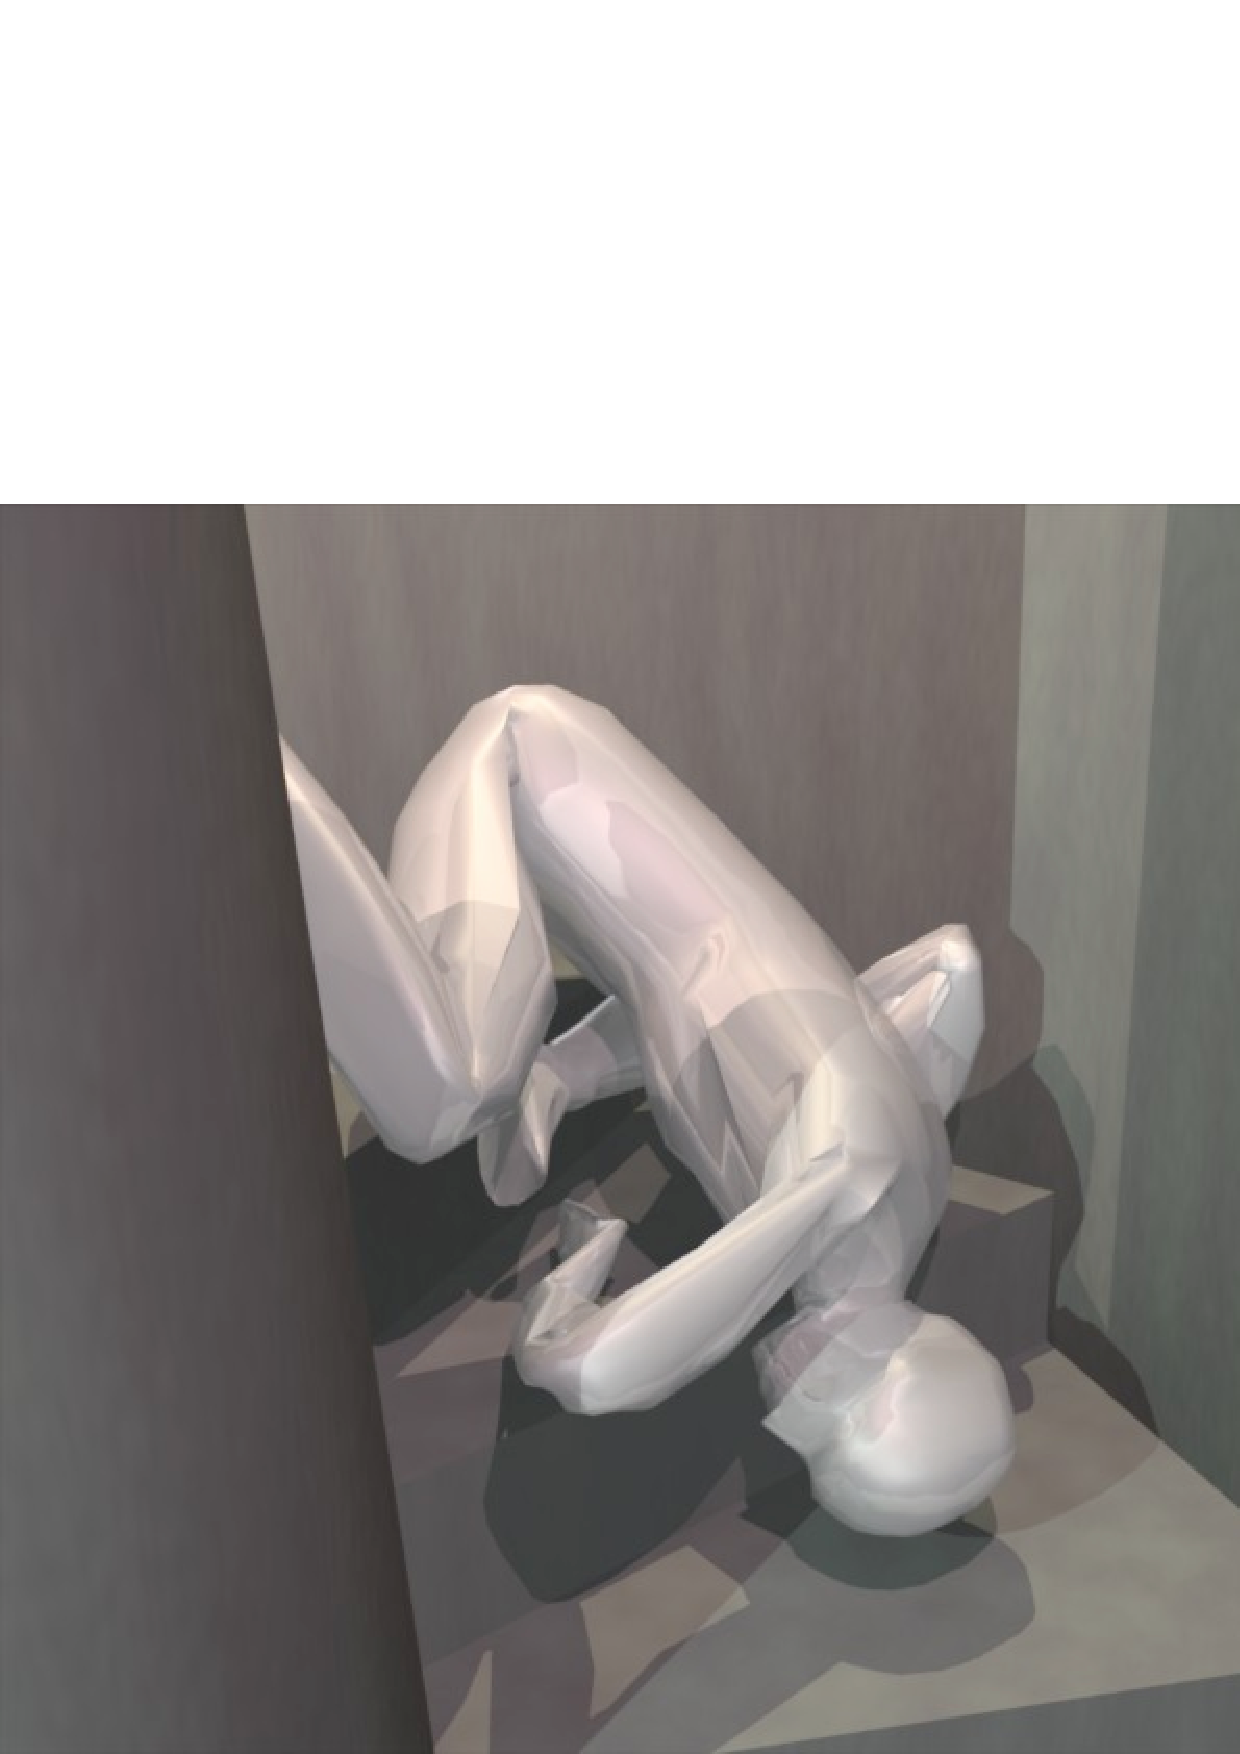
\includegraphics[width=60mm,height=45mm]{figures/spiral3} \hspace{5mm}
            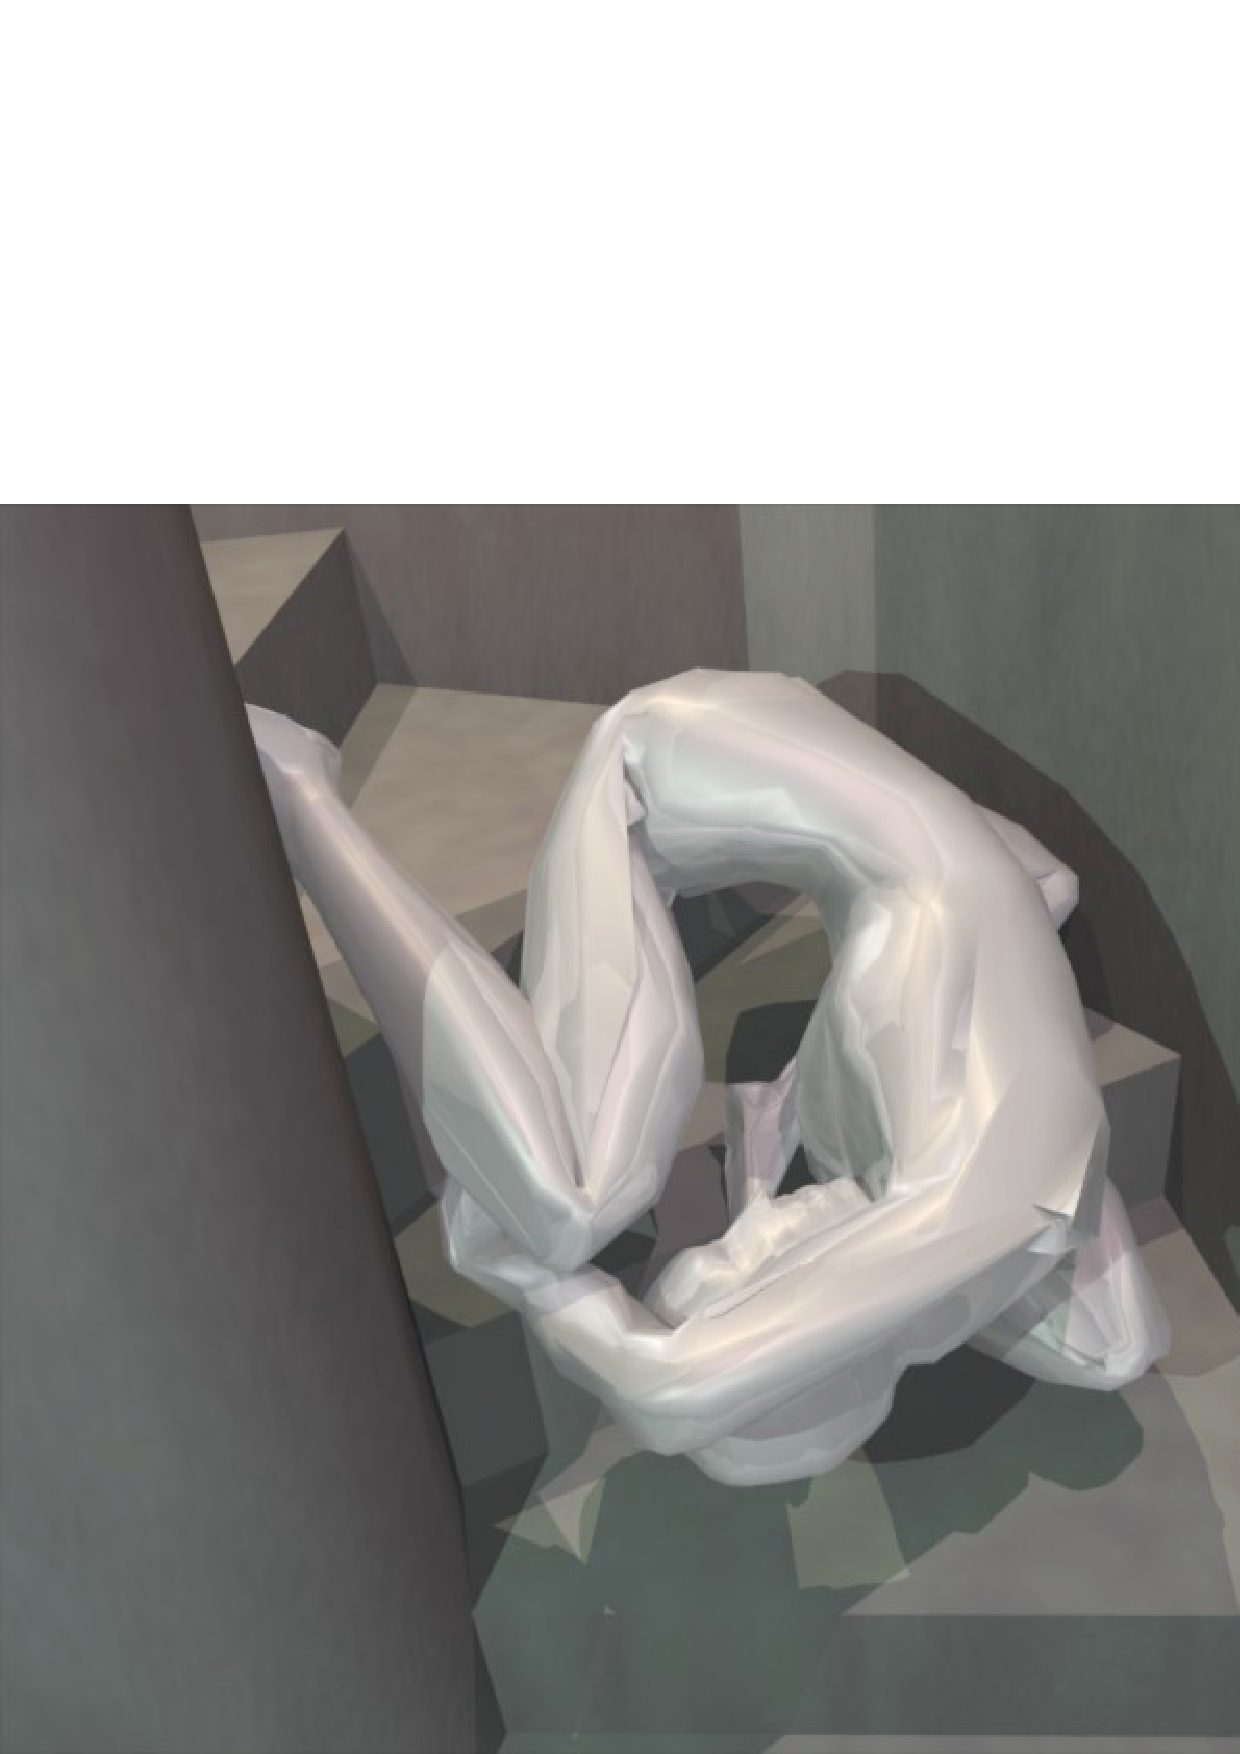
\includegraphics[width=60mm,height=45mm]{figures/spiral4}}
\caption{Animation of Alfred tumbling down a spiral staircase.\label{sampleSpiral}}
\end{figure}

